\documentclass[onecolumn, draftclsnofoot,10pt, compsoc]{IEEEtran}
\usepackage{graphicx}
\usepackage{url}
\usepackage{caption}
\usepackage{setspace}
\usepackage{listings}
\usepackage{color}

\usepackage{geometry}
\geometry{textheight=9.5in, textwidth=7in}
\usepackage{hyperref}

\definecolor{dkgreen}{rgb}{0,0.6,0}
\definecolor{gray}{rgb}{0.5,0.5,0.5}
\definecolor{mauve}{rgb}{0.58,0,0.82}

\usepackage{geometry}
\geometry{textheight=9.5in, textwidth=7in}

% 1. Fill in these details
\def \CapstoneTeamName{         Investment Performance Mobile Application}
\def \CapstoneTeamNumber{           68    }
\def \GroupMemberOne{                   Tyler Jones}
\def \GroupMemberTwo{                   Aviral Sinha}
\def \GroupMemberThree{                 Samuel Cooney}


% 2. Uncomment the appropriate line below so that the document type works
\def \DocType{          %Problem Statement
                                %Requirements Document
                                %Technology Review
                                Final Report
                                %Progress Report
                                }

\newcommand{\NameSigPair}[1]{\par
\makebox[2.75in][r]{#1} \hfil   \makebox[3.25in]{\makebox[2.25in]{\hrulefill} \hfill            \makebox[.75in]{\hrulefill}}
\par\vspace{-12pt} \textit{\tiny\noindent
\makebox[2.75in]{} \hfil                \makebox[3.25in]{\makebox[2.25in][r]{Signature} \hfill  \makebox[.75in][r]{Date}}}}
% 3. If the document is not to be signed, uncomment the RENEWcommand below
\renewcommand{\NameSigPair}[1]{#1}

%%%%%%%%%%%%%%%%%%%%%%%%%%%%%%%%%%%%%%%
\begin{document}
\begin{titlepage}
    \pagenumbering{gobble}
    \begin{singlespace}
       %\includegraphics[height=4cm]{}
        \hfill
        % 4. If you have a logo, use this includegraphics command to put it on the coversheet.
        %\includegraphics[height=4cm]{CompanyLogo}
        \par\vspace{.2in}
        \centering
        \scshape{
            \huge \DocType \par
            {\large\today}\par
            \vfill
            \vspace{5pt}
            \CapstoneTeamName\par
            \vspace{5pt}
            {\Large
                \NameSigPair{\GroupMemberOne}\par
                \NameSigPair{\GroupMemberTwo}\par
                \NameSigPair{\GroupMemberThree}\par
            }
            \vspace{20pt}
        }
        \begin{abstract}
        % 6. Fill in your abstract
        The purpose of this document is to describe in detail the Investment Performance Mobile Application. This document will break down the design and development of this application and includes all relevent documents and pieces of information that were used and created for this project.
        \end{abstract}
    \end{singlespace}
\end{titlepage}
\newpage
\pagenumbering{arabic}
\tableofcontents
% 7. uncomment this (if applicable). Consider adding a page break.
%\listoffigures
%\listoftables
\clearpage
\newpage
\pagenumbering{arabic}

\section{Introduction}

This project was created for Oregon State University's Computer Science Capstone class of 2017-18. The project idea was initially
created and sponsored by Hedge Serv's Brice Lemke with sponsorship continuing under Ronald Olshausen and Edison Tsai. The project sponsor's role
in  this project was a client who guided the project through the design of the scope of the project and assisted with
refocusing the scope throughout development. The team on this project was Samuel Cooney, Applied Computer Science
major with a minor in Business and Entrepreneurship, Tyler Jones, Applied Computer Science major with a minor in Mathematics, and Aviral Sinha, Applied Computer Science major with a minor in Economics.
The team designed, developed, and tested the project from start to finish, and took over sponsorship of the project in early April 2018.
Samuel Cooney was the front end expert and was responsible for all User Interface related work. Tyler Jones was the back end expert and was
responsible for all database, console, and API related work. Aviral Sinha was the financial expert and was responsible for ensuring financial
accuracy and accounting data work. 

\section{Requirements}
This section is broken into the initial requirements built for this application, and the updated requirements which was used for the final product.
\subsection{Initial Requirements}
\subsubsection{Purpose}
The purpose of this mobile application will be to provide it's users insight into the quality of their investments from a portfolio level. 
By using this application, a user will be able to track and gain valuable insight that wouldn't be possible otherwise.

\subsubsection{Scope}
The scope  of this project is to provide users with a method to track investment portfolios containing stocks and stock options. Users will have
the ability  to enter in investments and receive detailed tracking information on these assets. Data will be displayed including prices, purchase
dates, volatility, and more for both portfolio wide and individual investments.

\subsubsection{Definitions, acronyms, and abbreviations}
\begin{itemize}
	\item HedgeServ: A global, independent fund administration provider headquartered in New York with
		10 offices and 195+ clients worldwide.
	\item Xamarin: A tool built into Microsoft Visual Studio that allows developers to deliver native 
	   	C\# applications to Android, iOS, and Windows devices.
	\item C\#: (pronounced as \textit{see sharp}) is a programming language developed by Microsoft. It encompasses strong typing, imperative, declarative, functional, generic,
		object-oriented, and component-oriented programming styles.
	\item Asset: A valuable property such as resources, estate, holdings, etc...
	\item Investments: An asset or item purchased with the hope that it will generate income and is not consumed today and used to create wealth in the future.
	\item Portfolio: A group of financial assets that are held by investors or managed by financial professionals.
	\item Options: Contracts that grant the right but not obligation to buy or sell an underlying asset at a set price before a certain date.
	\item Front End: The view of an application that provides the end user with a friendly interface to interact with.
	\item Back End: The behind the scenes of an application that typically handles business logic and the storage of data.
	\item Domain-Specific Language: (Often referred to as \textit{DSL}) A programming language that has been specialized to a particular application domain.
	\item SQL: A domain-specific programming language used for managing data held in a database management system.
\end{itemize}

\subsubsection{Overview}

The Investment Performance Mobile Application will allow users to view their investment portfolio on iOS and Android devices
at a portfolio level. Users will receive data at a portfolio level as well as drill down to any of their specific investments.


\subsubsection{Product perspective}

Currently, most mobile financial applications provide investment performance information on only one investment type at a time. 
This project seeks to solve the current lack of a tool that concurrently tracks a variety of different investment assets in 
one consolidated source. In doing so, this application will allow users to place and view all of their investments in a single location 
while simultaneously receiving performance updates for each individual investment and the portfolio as a whole.

\subsubsection{Product Functions}
This mobile applciation will provide users investment performance from a portfolio level. The user will be able to enter investments, either 
in bulk or individually, and have their portfolio be displayed all together. Then users will have the ability to view different data
points about their portfolio as well as drill down into individual investments in order to get further data on a single asset.

While in the portfolio view, users will see a pie chart with their portfolio split up into percentages. 
For instance, if a user owns \$1000 worth of assets, these may be across stocks or stock options. A user may have \$500 invested in the stock market, 
and \$500 in a call option. The pie chart would reflect this division. Additionally, the user will be able to retrieve benchmarks on their entire portfolio. 
The S\&P 500, for example, would provide the user with a benchmark by which they could compare the performance of their entire portfolio against. 
Moreover, the user will be able to dissect the performance of their entire portfolio based off a variety of time intervals. The user will see the aggregate 
performance of their investments over time intervals ranging from a week all the way to multiple years+. Lastly, the user will be able to see their Sharpe ratio and volatility of their portfolio. 
The user will also be able to see all of this data at an individual investment level. This means that this applciation should provide the user 
time data, the Sharpe ratio, volatility, and benchmarks of individual investments, when relevant/available.


\subsubsection{Specific requirements}

\paragraph{Backend}

\begin{itemize}
\item There must be no longer than a 3 second response time on any given query to the database. If queries fail, the data should be blank or missing, 
		rather than inaccurate. Users should be able to rely on 100\% accurate pricing data, even if not 100\% up to date; inaccurate pricing is not an option. Crashing is better than showing incorrect data, however this crash rate should be low. Moreover, the crash rate will be measured as the number of crashes relative to the number of queries to the database, rather than crashes relative to unit time.

\item Database must be able to accommodate users having more than one portfolio/account
\item Database must be able to accommodate users having a joint portfolio/investment.
\item All transactions must be stored in the database
\item The final product must be secure. Usernames and passwords must be safely stored in the database, and prevent hacking attempts such as SQL injections.
\item Investment prices stored in the database should be automatically updated daily and store old data so that portfolios can track historical data.
\end{itemize}

\paragraph{Frontend}
\begin{itemize}
	\item Front end development will be written in C\#, and SQL will be used for the back-end. Various API's can be used to receive data from Internet sources.  
	\item Investments must be able to be removed from the portfolio, as the user should 
		have complete control over what they track. 
	\item Portfolio level will allow the user to see a pie chart of their total assets with each section being an individual investment.
	\item The portfolio will have relative benchmarks to industry standard sources like the S\&P500.
	\item An option to view the portfolio's history in a graph must be displayed with a variety of time intervals ranging from a day to weeks to multiple years.
	\item The portfolio should display the current Sharpe Ratio as well as its volatility.
	\item Individual investments should also track time data, Sharpe Ratio, Volatility, and relative benchmarks when relevant/available separate from the portfolio benchmarks.
	\item Users must be able to enter data through the application in two formats. First, one investment at a time manually added in using the user-friendly interface. Second by
		adding a CSV file or EXCEL file containing the user's portfolio data to the application will automatically populate the user's profile based off the contents of said file.
	\item Investments should list purchase price and quantity, at a minimum.
	\item Both the portfolio and individual investments should show returns based off time and purchase price.
	\item User's portfolio should be cached onto the device when the user logs in.
	\item Stock splits should properly increase investment quantity and reduce price when such event occurs (investment value should remain unchanged).

	
\end{itemize}
\subsubsection{Timeline}
Attached below.

\begin{figure}[h]
\centering
\captionsetup{justification=centering}
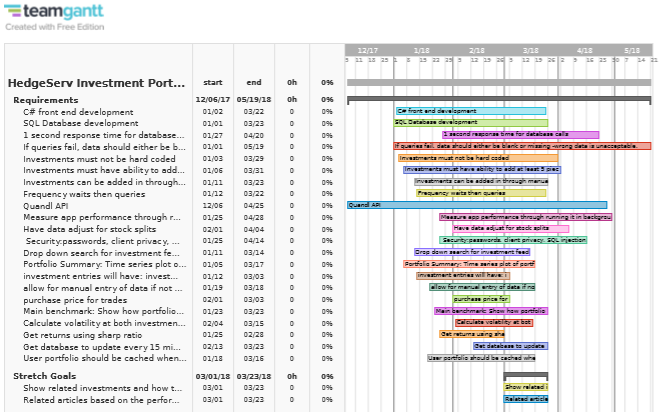
\includegraphics[width=7in]{require/ganttchart.PNG}
\caption{Gantt Chart}
\end{figure}

\newpage
\subsection{Updated Requirements - March 15, 2018}

\subsubsection{Purpose}
The purpose of this mobile application will be to provide it's users insight into the quality of their investments from a portfolio level. 
By using this application, a user will be able to track and gain valuable insight that wouldn't be possible otherwise.

\subsubsection{Scope}
The scope  of this project is to provide users with a method to track investment portfolios containing stocks. Users will have the ability  to enter in investments and receive detailed tracking information on these assets. Data will be displayed including prices, purchase dates, volatility, and more for both portfolio wide and individual investments.

\subsubsection{Definitions, acronyms, and abbreviations}
\begin{itemize}
	\item HedgeServ: A global, independent fund administration provider headquartered in New York with
		10 offices and 195+ clients worldwide.
	\item Xamarin: A tool built into Microsoft Visual Studio that allows developers to deliver native 
	   	C\# applications to Android, iOS, and Windows devices.
	\item C\#: (pronounced as \textit{see sharp}) is a programming language developed by Microsoft. It encompasses strong typing, imperative, declarative, functional, generic,
		object-oriented, and component-oriented programming styles.
	\item Asset: A valuable property such as resources, estate, holdings, etc...
	\item Investments: An asset or item purchased with the hope that it will generate income and is not consumed today and used to create wealth in the future.
	\item Portfolio: A group of financial assets that are held by investors or managed by financial professionals.
	\item Front End: The view of an application that provides the end user with a friendly interface to interact with.
	\item Back End: The behind the scenes of an application that typically handles business logic and the storage of data.
	\item Domain-Specific Language: (Often referred to as \textit{DSL}) A programming language that has been specialized to a particular application domain.
	\item SQL: A domain-specific programming language used for managing data held in a database management system.
\end{itemize}

\subsubsection{Overview}

The Investment Performance Mobile Application will allow users to view their investment portfolio on iOS and Android devices at a portfolio level. Users will receive data at a portfolio level as well as drill down to any of their specific investments.


\subsubsection{Product perspective}

Currently, most mobile financial applications provide investment performance information on only one investment type at a time. This project seeks to solve the current lack of a tool that concurrently tracks a variety of different investment assets in  one consolidated source. In doing so, this application will allow users to place and view all of their investments in a single location while simultaneously receiving performance updates for each individual investment and the portfolio as a whole.

\subsubsection{Product Functions}
This mobile application will provide users investment performance from a portfolio level. The user will be able to enter investments, either  in bulk or individually, and have their portfolio be displayed all together. Then users will have the ability to view different data points about their portfolio as well as drill down into individual investments in order to get further data on a single asset.

While in the portfolio view, users will see a pie chart with their portfolio split up into percentages. 
For instance, if a user owns \$1000 worth of assets, these may be across different stocks and the pie chart will reflect this division. Additionally, the user will be able to retrieve benchmarks on their entire portfolio. The S\&P 500 or Dow Jones Index, for example, would provide the user with a benchmark by which they could compare the performance of their entire portfolio against.  Moreover, the user will be able to dissect the performance of their entire portfolio based off a variety of time intervals. The user will see the aggregate 
performance of their investments over time intervals ranging from a week all the way to multiple years+. Lastly, the user will be able to see their Sharpe ratio and volatility of their portfolio. 
The user will also be able to see all of this data at an individual investment level. This means that this application should provide the user financial ratios, investment level balance sheets, income statements, and cash flows. We would also show how the portfolio against benchmarks specifically against index funds that track the market as a whole. 


\subsubsection{Specific requirements}

\paragraph{Backend}

\begin{itemize}
\item There must be no longer than a 3 second response time on any given query to the database. If queries fail, the data should be blank or missing,rather than inaccurate. Users should be able to rely on 100\% accurate pricing data, even if not 100\% up to date; inaccurate pricing is not an option. Crashing is better than showing incorrect data, however this crash rate should be low. Moreover, the crash rate will be measured as the number of crashes relative to the number of queries to the database, rather than crashes relative to unit time.

\item Database must be able to accommodate users having more than one portfolio/account
\item Database must be able to accommodate users having a joint portfolio/investment.
\item All transactions must be stored in the database
\item The final product must be secure. Usernames and passwords must be safely stored in the database, and prevent hacking attempts such as SQL injections. 
\item Investment prices stored in the database should be automatically updated regularly and store old data so that portfolios can track historical data. 
\end{itemize}

\paragraph{Frontend}
\begin{itemize}
	\item Front end development will be written in C\# through Xamarin Forms which allows for cross platform compatibility. 
	\item Investments must be able to be removed from the portfolio, as the user should 
		have complete control over what they track. 
	\item Portfolio level will allow the user to see a pie chart of their total assets with each section being an individual investment.
	\item The portfolio will have relative benchmarks to industry standard sources like the S\&P500.
	\item An option to view the portfolio's history in a graph must be displayed with a variety of time intervals ranging from a day to weeks to multiple years.
	\item The portfolio should display the current Sharpe Ratio as well as its volatility.
	\item Users must be able to enter data through the application one investment at a time manually added in using the user-friendly interface. 
	\item Investments should list purchase price and quantity, at a minimum.
	\item Both the portfolio and individual investments should show returns based off time and purchase price.
	\item Stock splits should properly increase investment quantity and reduce price when such event occurs (investment value should remain unchanged).

	
     \end{itemize}

\newpage




\section{Design}

This section is broken down into the initial design document built for this application, and the updated design document which was used for the final product.
\subsection{Initial Design Document}
\subsubsection{Introduction}

    The following sections will cover the main design elements of the Investment Performance Mobile
    Application for HedgeServ. This document will also go over the various technologies and tools being implemented and their
    relationship with each other. As a disclaimer, this application will be a student made learning tool and is in
    no way recommended as a tool  to make financial decisions from. As the members of this team are still in early stages of development,
    not everything mentioned in this document will be rigid. 
      
\begin{table}[h]
                        \caption{Table 1 - Summary of Design Viewpoints}
                        \centering
                                \begin{tabular}{| p{0.3\linewidth} | p{0.3\linewidth} | }
                                        \hline
                                         \textbf{Design Viewpoint} & \textbf{Design Concerns}\\ [0.5ex]
                                        %heading
                                        \hline
                                        Context(Section 2)  & Systems services and users\\
                                        \hline
                                         Composition(Section 3) & Composition and modular assembly of systems in terms of subsystems\\
                                        \hline
                                         Logical(Section 4) & Static structure\\
                                        \hline
                                        Dependency(Section 5) & Interconnection, sharing, and parameterization\\
                                        \hline
                                        Information(Section 6) & Persistent information\\
                                        \hline
                                        Interface(Section 7) & Service definition and access\\
                                        \hline
                                \end{tabular}
\end{table}     


\subsubsection{Context viewpoint}
        This financial mobile application aims to supplement users' investment experience by providing insight into the quality of investments from a individual and portfolio level.
        Relevant stakeholders include the developers of this application, namely Tyler Jones, Avi Sinha, and Sam Cooney, as well as HedgServe employees namely Edison Tsai and Ronald Olshausen.

        From a "black box" perspective, the application will allows users to enter an investment, including type of asset class, either stock or stock option, company name and ticker symbol,
        and amount invested combined with shares purchased. The user will then have proper pricing data displayed for the investment for a given time period, and the portfolio and individual
        investments will display the performance of the user's investments based on such pricing.

\paragraph{Design concerns}
        The scope and use of this application is to be a learning tool, both for the relevant developers, as well as any future users. Typically, in an enterprise environment, many audits and
        checkpoints must be performed on the application in order to verify it as a reliable source of financial advice. Due to the time span and scope of this application, such regulation and
        checkpoints are not going to be made, and as such, this application is not intended for the purpose of either handling real finances, nor to be used to make fully informed financial decisions.
        Any relevant statistics displayed for the user based on their current investments should be investigated more in depth by said user.

\paragraph{Design Elements}
        Design entities: Actors - A MySQL database will be interacting directly with the front end of the application, and thus the user. When a user enters a new investment into the application
        through the UI, said entry is stored in the MySQL database and can later be retrieved as the user needs. Moreover, API calls through Quandl will be made that allow the users stored investment
        information to have relevant pricing data displayed.

\subsubsection{Composition viewpoint}
\paragraph{Design Elements}
        Design Entities: The investment performance mobile application can be broken down in 4 primary components/entities. These components are the user interface, the database, API, and Development Tools.

\paragraph{Design Relationships}
        The database, and chosen financial data API both will work with the user interface. The database will contain the financial information that was entered by the user, and the API will
        supplement such data with relevant pricing info in order to give performance metrics. Both the API and database will be displayed on the front end of the application, and will appear
        to the user in a desirable fashion through the interface.

\paragraph{Function Attribute: APIs}
        This application will be handling various data sets that need to be constantly pulled and updated. Instead of manually uploading individual sets, Quandl will be utilized as recommended by HedgeServ. Through Quandl,
	various financial, economic, and alternative data will be accessible. The API will be used in a python like environment where a vast array of free data sets provided by many reputable sources are open for use.
	Since HedgeServ primarily serves buy side firms that not only look at typical investments like stocks and options but alternative investments that may prove useful in the future if the application wants to expand
	beyond what is outlined in the original scope. 
        
        Portfolio data will also need to be visualized through charts and graphs that allow the user to quickly glance at an investment. The visualizations will show historical investment prices as well as other
	variables related to that security. Since this will be an application for both Android and iOS a visualization tool that would be supported by both platforms is required. Google Charts will allow portfolio data to
	be shown in a visually appealing manner using various libraries, resources, and tools. 
        
\paragraph{Function Attribute: User Interface}
        The user interface will all be handled through Android and iOS devices. Users must be able to quickly and
        securely log into their account and be loaded to the dashboard. From here, the user can select a specific
        portfolio to look at, create a new individual or shared portfolio, or edit account information.
        When selecting a portfolio, the user can see information and statistics on their portfolio in the 
        form of charts, graphs, history displays, and data tables. The portfolio view will also allow users to edit their
        portfolio by adding or removing stocks and stock options. By selecting a specific option or stock on the
        pie chart, users can see individual information on the stock including purchase price(s), current price,
        and purchase date.
        
\paragraph{Function Attribute: Database}
        The database will hold the financial data that was entered by the user. This database will be a relational database that is hosted by Oregon State University. Such a choice was
        made due to the financial advantage that using this database provides. Every student at the university is given 1 free database, and for this reason it was chosen. The database
        management system that will be used is MySQL.

        The database will contain not only financial data, but will also contain login information, and the number of portfolios that belong to a specified user. A user can share a portfolio
        with another user, as well as have an individual portfolio. In the case of joint custody, the two users will both be able to retrieve and access the portfolio from their interface.
        A relational database, such as the one that will be implemented, is perfect for this purpose.

\paragraph{Function Attribute: Development Tools}
    As recommended by HedgeServ, Xamarin will be the main tool for development to ensure a smooth and efficient development process. Its native libraries make use of C\# and .NET to allow cross platform
    development which will be key with the utilization of various data tools. The Investment Performance Mobile Application requires the ability to develop cross platform easily without losing 
    application performance. By having a platform specific UI the application will look at home on both iOS and Android with specific design cues and functions. Thanks to Xamarin's open source technology,
    compatibility with most APIs will be ensured and eliminate the risk of having to go back to the drawing board when implementing a crucial part of the application. The use of a single stack will allow 
    a quick time to market which means simultaneously running testing on various versions while continuing development. By using Xamarin, the development process will be streamlined to ensure the final product
    is fully functional and visually appealing for HedgeServ. 


\subsubsection{Logical viewpoint}
        Various other financial applications were researched for influence in the design of this application. Most notably Robinhood which makes use of a mobile friendly user interface which allows the user to
	easily buy and sell stocks, look at historical data, other info, and news related to the investment's industry. Their model is built on the goal to appeal to a mobile generation that needs all of their
	investments on the go. Even though this project is meant to be a learning tool and is not intended to be released as a HedgeServ product, ensuring the highest quality will be intended in the development
	of this application. This holds especially true for industry leaders like Robinhood and Merrill Edge who have essentially made consumer versions of what was once only available to trading firms. 
     
\subsubsection{Dependency viewpoint}

      For the most part all of the design tools will be heavily dependent on each other. This project is relatively small in scale due it mainly being a mobile application. This project can be broken down into four main
      sections: APIs, User Interface, Database, and Development Tools. These consist of what our application will actually be in addition what is required to make the end product possible. Without the various APIs this
      application won't be able to properly get the data sets nor visualize it and the database allows for all the vast amount of data to come in from Quandl and be organized in a fashion that allows the user to easily access the
      information they need. These all depend on a working user interface because while there may be tables with thousands of data points it will all be somewhat useless in the context of this project the application is not
      navigable and intuitive. All of this relies on the strong foundation Xamarin provides which is the main development tool and the primary ecosystem for all aspects of the application development. 

\subsubsection{Information viewpoint}

        User financial data will be stored in a MySQL database. This section intends on going into more detail
        about the implementation and expectation of stored
        data based on what the user will be able to enter from within the user interface.

        At this point in time, the user will be able to provide the following to the application, and will contain two primary types of tables:

\paragraph{User Table}
\begin{itemize}
    \item Login information that is encrypted. Encryption will likely be done with either SHA1 or SHA256.
    \item Portfolios held. This will be stored as an integer.
    \item Names of portfolios. Portfolios named will contain a foreign key relating to the proper portfolio within the portfolio table.
\end{itemize}
\paragraph{Portfolio Table}
\begin{itemize}
    \item Owners of the portfolio. Can be owned by multiple users, or one user.
    \item Total amount invested in USD. This will be stored as a floating point number.
    \item Amount invested per company
    \item Number of shares purchased based on amount invested. This will be stored as a floating point number.
    \item Types of investments, either a stock or stock option. This can be stored as either a string, or because only two asset classes are supported, perhaps a binary value to represent the type (0 or 1).
    \item Ticker Symbol of company invested. This will be stored as a string.

\end{itemize}

\begin{figure}[h]
\centering
\captionsetup{justification=centering}
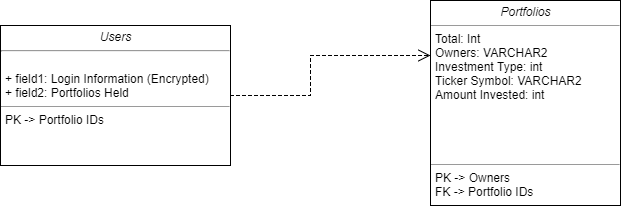
\includegraphics[width=14cm]{design/database.png}
\caption{UML Database Diagram}
\end{figure}

%Every application, however trivial, uses patterns. Some patterns even include things like committing code every
%line change or using automated testing during releases. 
%\section{Patterns use viewpoint}
%Our application will be very intuitive in design which means that we will be using similar patterns in %functionality and design throughout and won't differ heavily. 

\subsubsection{Interface viewpoint}

    Interface viewpoint outlines how three of the core functions interface and interact with one another.
    Beginning with the user interface where portfolio owners can add and remove stocks and options which
    sends updates to the database where the data is stored. The portfolio view also has graphs, charts, history displays,
    and data tables which will be retrieved from various APIs including websites like Quandl and Google Finance.
    
\paragraph{Design Elements}
    \begin{itemize}
        \item User Interface
        \item APIs
        \item Database
    \end{itemize}

\paragraph{Interface Attributes}

    The user interface is the mobile application that will be used as a front end display for portfolios. Most
    interactions will come from this section, instead of getting called to. Databases will send back information
    regarding account info, portfolio data and ownership, and log in. The web services like Quandl and Google 
    Finance will also send response data to the mobile application which can then process that data into charts 
    and other forms of processable information.

\begin{figure}[h]
\centering
\captionsetup{justification=centering}
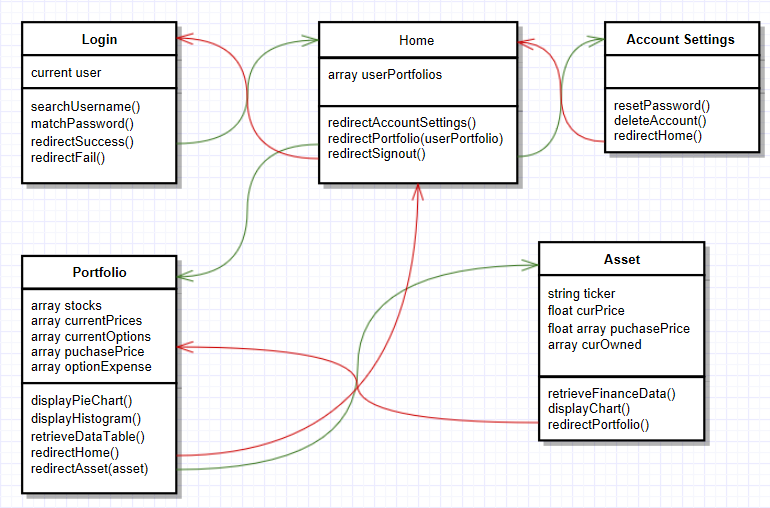
\includegraphics[width=14cm]{design/frontend.png}
\caption{UML User Interface Diagram}
\end{figure}
    
    The web services and APIs that will be connected to our application will mainly be called from the user
    interface. When a portfolio attempts to display a history display of stock prices, calls will be made from the user
    interface to a wrapper for Quandl's API. Periodically, the web service will make calls to the APIs and 
    then report this information to the database. This will continually keep our database's information
    up to date which allows for quicker loading on the front end.
    
    The database will be a strong point of interaction in our project. The user interface will interact heavily
    post log in of a user as the application will load all the information on a specific user's portfolios and their
    data. The application will also add or remove information to the database with calls when the user is adding 
    a new stock or option or removing one of the two asset classes. The web services will also be connecting
    to the database periodically to update its information on stock prices or stock splits.

\newpage
\subsection{Updated Design Document - March 15, 2018}
\subsubsection{Introduction}

    The following sections will cover the main design elements of the Investment Performance Mobile
    Application for HedgeServ. This document will also go over the various technologies and tools being implemented and their
    relationship with each other. As a disclaimer, this application will be a student made learning tool and is in
    no way recommended as a tool  to make financial decisions from. As the members of this team are still in early stages of development,
    not everything mentioned in this document will be rigid. 
      
\begin{table}[h]
                        \caption{Table 1 - Summary of Design Viewpoints}
                        \centering
                                \begin{tabular}{| p{0.3\linewidth} | p{0.3\linewidth} | }
                                        \hline
                                         \textbf{Design Viewpoint} & \textbf{Design Concerns}\\ [0.5ex]
                                        %heading
                                        \hline
                                        Context(Section 2)  & Systems services and users\\
                                        \hline
                                         Composition(Section 3) & Composition and modular assembly of systems in terms of subsystems\\
                                        \hline
                                         Logical(Section 4) & Static structure\\
                                        \hline
                                        Dependency(Section 5) & Interconnection, sharing, and parameterization\\
                                        \hline
                                        Information(Section 6) & Persistent information\\
                                        \hline
                                        Interface(Section 7) & Service definition and access\\
                                        \hline
                                \end{tabular}
\end{table}     


\subsubsection{Context viewpoint}
        This financial mobile application aims to supplement users' investment experience by providing insight into the quality of investments from a individual and portfolio level.
        Relevant stakeholders include the developers of this application, namely Tyler Jones, Avi Sinha, and Sam Cooney, as well as HedgServe employees namely Edison Tsai and Ronald Olshausen.

        From a "black box" perspective, the application will allows users to enter an investment, in this case a stock, the company name, its ticker symbol,
        and amount invested combined with shares purchased. The user will then have proper pricing data displayed for the investment for a given time period, and the portfolio and individual
        investments will display the performance of the user's investments based on such pricing.

\paragraph{Design concerns}
        The scope and use of this application is to be a learning tool, both for the relevant developers, as well as any future users. Typically, in an enterprise environment, many audits and
        checkpoints must be performed on the application in order to verify it as a reliable source of financial advice. Due to the time span and scope of this application, such regulation and
        checkpoints are not going to be made, and as such, this application is not intended for the purpose of either handling real finances, nor to be used to make fully informed financial decisions.
        Any relevant statistics displayed for the user based on their current investments should be investigated more in depth by said user.

\paragraph{Design Elements}
        Design entities: Actors - A MySQL database will be interacting directly with the front end of the application, and thus the user. When a user enters a new investment into the application
        through the UI, said entry is stored in the MySQL database and can later be retrieved as the user needs. Moreover, API calls through Alpha Vantage and Last10K will be made that allow the users stored investment
        information to have relevant pricing data displayed.

\subsubsection{Composition viewpoint}
\paragraph{Design Elements}
        Design Entities: The investment performance mobile application can be broken down in 4 primary components/entities. These components are the user interface, the database, API, and Development Tools.

\paragraph{Design Relationships}
        The database, and chosen financial data API both will work with the user interface. The database will contain the financial information that was entered by the user, and the API will
        supplement such data with relevant pricing info in order to give performance metrics. Both the API and database will be displayed on the front end of the application, and will appear
        to the user in a desirable fashion through the interface.

\paragraph{Function Attribute: APIs}
        This application will be handling various data sets that need to be constantly pulled and updated. Instead of manually uploading individual sets, Alpha Vantage and Last10k will be utilized. Through these API's various financial, economic, and alternative data will be accessible. The two API's will be integrated together where we will be parsing the data to show what is required for the user. Which include various financial ratios, balance sheets, income statements, and cash flow. 
        Portfolio data will also need to be visualized through charts and graphs that allow the user to quickly glance at an investment. The visualizations will show historical investment prices as well as other variables related to that security. Since this will be an application for both Android and iOS a visualization tool that would be supported by both platforms is required. Xamarin Forms allows integration with an internal API which will allow portfolio data to	be shown in a visually appealing manner using various libraries, resources, and tools. 
        
\paragraph{Function Attribute: User Interface}
        The user interface will all be handled through Android and iOS devices. Users must be able to quickly and
        securely log into their account and be loaded to the dashboard. From here, the user can select a specific
        portfolio to look at, create a new individual or shared portfolio, or edit account information.
        When selecting a portfolio, the user can see information and statistics on their portfolio in the 
        form of charts, graphs, history displays, and data tables. The portfolio view will also allow users to edit their
        portfolio by adding or removing stocks. By selecting a specific stock on the
        pie chart, users can see individual information on the stock including purchase price(s), current price,
        and purchase date.
        
\paragraph{Function Attribute: Database}
        The database will hold the financial data that was entered by the user. This database will be a relational database that is hosted by Oregon State University. Such a choice was
        made due to the financial advantage that using this database provides. Every student at the university is given 1 free database, and for this reason it was chosen. The database
        management system that will be used is MySQL.

        The database will contain not only financial data, but will also contain login information, and the number of portfolios that belong to a specified user. A user can share a portfolio
        with another user, as well as have an individual portfolio. In the case of joint custody, the two users will both be able to retrieve and access the portfolio from their interface.
        A relational database, such as the one that will be implemented, is perfect for this purpose.

\paragraph{Function Attribute: Development Tools}
    As recommended by HedgeServ, Xamarin will be the main tool for development to ensure a smooth and efficient development process. Built within Visual Studio, Xamarin's cross platform tool known as Xamarin Forms will allow native libraries to make use of C\# and .NET for cross platform development which will be key with the utilization of various data tools. The Investment Performance Mobile Application requires the ability to develop cross platform easily without losing application performance. By having a platform specific UI the application will look at home on both iOS and Android with specific design cues and functions. Thanks to Xamarin's open source technology,compatibility with most APIs will be ensured and eliminate the risk of having to go back to the drawing board when implementing a crucial part of the application. The use of a single stack will allow a quick time to market which means simultaneously running testing on various versions while continuing development. By using Xamarin, the development process will be streamlined to ensure the final product is fully functional and visually appealing for HedgeServ. 


\subsubsection{Logical viewpoint}
        Various other financial applications were researched for influence in the design of this application. Most notably Robinhood which makes use of a mobile friendly user interface which allows the user to easily buy and sell stocks, look at historical data, other info, and news related to the investment's industry. Their model is built on the goal to appeal to a mobile generation that needs all of their investments on the go. Even though this project is meant to be a learning tool and is not intended to be released as a HedgeServ product, ensuring the highest quality will be intended in the development of this application. This holds especially true for industry leaders like Robinhood and Merrill Edge who have essentially made consumer versions of what was once only available to trading firms. 
     
\subsubsection{Dependency viewpoint}

      For the most part all of the design tools will be heavily dependent on each other. This project is relatively small in scale due it mainly being a mobile application. This project can be broken down into four main
      sections: APIs, User Interface, Database, and Development Tools. These consist of what our application will actually be in addition what is required to make the end product possible. Without the various APIs this
      application won't be able to properly get the data sets nor visualize it and the database allows for all the vast amount of data to come in from the APIs and be organized in a fashion that allows the user to easily access the
      information they need. These all depend on a working user interface because while there may be tables with thousands of data points it will all be somewhat useless in the context of this project the application is not
      navigable and intuitive. All of this relies on the strong foundation Xamarin provides which is the main development tool and the primary ecosystem for all aspects of the application development. 

\subsubsection{Information viewpoint}

        User financial data will be stored in a MySQL database. This section intends on going into more detail
        about the implementation and expectation of stored
        data based on what the user will be able to enter from within the user interface.

        At this point in time, the user will be able to provide the following to the application, and will contain two primary types of tables:

\paragraph{User Table}
\begin{itemize}
    \item Login information that is encrypted. Encryption will likely be done with either SHA1 or SHA256.
    \item Portfolios held. This will be stored as an integer.
    \item Names of portfolios. Portfolios named will contain a foreign key relating to the proper portfolio within the portfolio table.
\end{itemize}
\paragraph{Portfolio Table}
\begin{itemize}
    \item Owners of the portfolio. Can be owned by multiple users, or one user.
    \item Total amount invested in USD. This will be stored as a floating point number.
    \item Amount invested per company
    \item Number of shares purchased based on amount invested. This will be stored as a floating point number.
    \item Ticker Symbol of company invested. This will be stored as a string.

\end{itemize}

\begin{figure}[h]
\centering
\captionsetup{justification=centering}
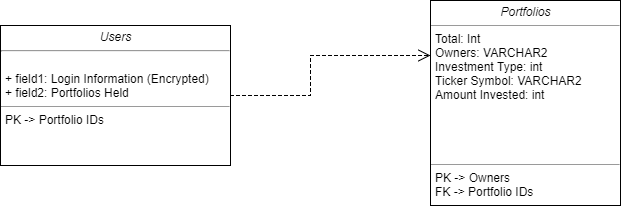
\includegraphics[width=14cm]{design/database.png}
\caption{UML Database Diagram}
\end{figure}

\subsubsection{Interface viewpoint}

    Interface viewpoint outlines how three of the core functions interface and interact with one another.
    Beginning with the user interface where portfolio owners can add and remove stocks which sends updates to the database where the data is stored. The portfolio view also has graphs, charts, history displays,
    and data tables which will be retrieved from Alpha Vantage, Last10k, and the main database we are hosting. 
    
\paragraph{Design Elements}
    \begin{itemize}
        \item User Interface
        \item APIs
        \item Database
    \end{itemize}

\paragraph{Interface Attributes}

    The user interface is the mobile application that will be used as a front end display for portfolios. Most
    interactions will come from this section, instead of getting called to. Databases will send back information
    regarding account info, portfolio data and ownership, and log in. The web services like Last10k and Alpha Vantage
     will also send response data to the mobile application which can then process that data into charts 
    and other forms of processable information.

\begin{figure}[h]
\centering
\captionsetup{justification=centering}
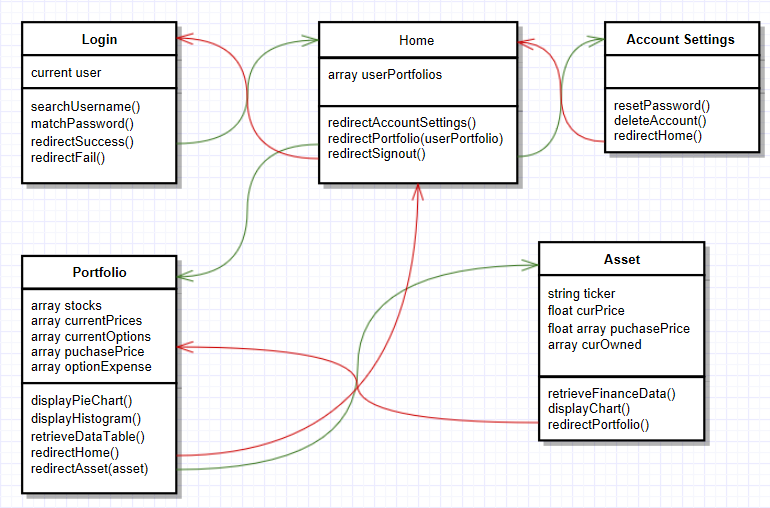
\includegraphics[width=14cm]{design/frontend.png}
\caption{UML User Interface Diagram}
\end{figure}
    
    The web services and APIs that will be connected to our application will mainly be called from the user
    interface. When a portfolio attempts to display a history display of stock prices, calls will be made from the user
    interface to a wrapper for our APIs. Periodically, the web service will make calls to the APIs and 
    then report this information to the database. This will continually keep our database's information
    up to date which allows for quicker loading on the front end.
    
    The database will be a strong point of interaction in our project. The user interface will interact heavily
    post log in of a user as the application will load all the information on a specific user's portfolios and their
    data. The application will also add or remove information to the database with calls when the user is adding 
    a new stock or removing one of the two asset classes. The web services will also be connecting to the database periodically to update its information on stock prices or stock splits.






\section{Tech Review}
\subsection{Introduction}

The Investment Performance Mobile Application is at a broad view a tool users will be able to track and receive insightful data about their asset portfolios. Users will be have the ability
to track stocks and stock options through their mobile devices using either iOS and Android phones. The application will connect to web services to run calculations on information it is retrieving from the database.
My role in this project will  be to develop the front end of the application which entails creating all the 
interfaces that the user will interact with as well as implementing the connections to the web services.

\subsection{Development Platform}
\subsubsection{Overview}
Development platforms are one of the foundations to creating a strong and secure application. Every development platform has its benefits and downsides, and choosing
one before beginning design can limit the decisions that will be made during development. Some development platforms can easily be integrated with other tools like Git for
version control, native device APIs for increased integration to mobile platforms, and various open-sources iOS and Android libraries that have numerous capabilities that give increased
functionality. These integrations as well as the platforms base abilities have to be weighed before selection or there could be walls that are run into during development.

\subsubsection{Criteria}
Development platforms will be compared on the following criteria:
\begin{itemize}
	\item Developed code can be shared on both iOS and Android devices. Our project is required to deploy onto both of these platforms, and so the tool needs match the job.
	\item Free to Use. There  is no funding for our project, so we need free software that we can work with that will not inhibit our work cycle.
	\item Git Integration. Our code lives on an external GitHub repository and since we are working as a team, quick roll-outs to our code base need to be made seamlessly.
	\item Code Compiler. The development platform needs to be able to compile our code for deployment, without this the code is not usable.
\end{itemize}
\subsubsection{Potential Choices}
\paragraph{Xamarin}

Xamarin is a development platform built with the goal of writing native Android, iOS, and Windows applications with a shared code base. Microsoft acquired Xamarin 
in February of 2016 in which they open-sourced the Xamarian SDK and bundled it within Visual Studio, another Microsoft product. Visual Studio Community is free
which allows the development within Xamarin for no cost. Development code is written in C\# which allows for sharing a single code base across the different platforms.
Xamarin also has built-in compilers that generate the platform specific needs: ARM assembly for iOS, IL with packaging by MonoVM and JIT'ing for Android, and IL for Windows.
However, Xamarin does remove some classes from various frameworks during compilation which could decrease usability. Visual Studio Community does have Git built directly into the IDE.
This allows for quicker saving of changes and removes the need for exiting the development platform to push changes to a remote repository. This is advantageous when working with
a team as well as keeping a change log for possible rollbacks. Overall, Xamarin meets all criteria with the only downside being possible loss of features when compiling.

\paragraph{PhoneGap}

PhoneGap is an open source framework built on Cordova and is owned by Adobe. It allows for development of hybrid mobile applications using HTML, CSS, and Javascript and a single code base.
Since PhoneGap is open source, the platform is free to use with an easy application install that also comes with a Developer Application that gives the ability to preview the applications on a desktop.
Adobe offers services alongside the framework that make PhoneGap a powerful tool, the Developer App being one of these add on services. PhoneGap Build is another service that allows developers to
compile their applications on cloud services. This removes the need to configure manual environments for compilation on each platform. PhoneGap unfortunately does not have any built in Git integration
which forces the need to use a separate tool to save and push changes to a remote repository. Overall, the base PhoneGap meets half of the requirements missing the Git integration and some
of the services the Adobe offers to make this a full tool have high subscription costs.

\paragraph{MonoCross}

MonoCross is an open source framework that uses C\#, .NET, and the Mono framework to give developers the ability to create cross platform mobile applications. Development with MonoCross is
done in C\# with full access to native device APIs. MonoCross also supports development in HTML, CSS, and JavaScript for hybrid web applications for developers who have a strong web background.
MonoCross is free to use and can be integrated into Visual Studio.
Since Visual Studio is free, this gives developers the ability to compile their code for all platforms without having to leave their development environment. This also allows for the ability to have built in Git
integration which removes the need to swap applications to save and push changes to a remote repository. Overall, MonoCross meets all of the requirements with the biggest downside being that the product
is not developed directly for Visual Studio.

\subsubsection{Discussion}

Comparing the three development platforms, one stands out clearly as being weaker than the rest, PhoneGap. 
PhoneGap requires additional services from Adobe to bring in the same capabilities that MonoCross and Xamarin bring to the table. It requires the use of PhoneGap Build, a cloud service building environment,
which causes the developer to purchase a subscription to Adobe to compile their code. This and the lack of Git integration makes PhoneGap a poor choice for the development platform.
The other potential choices, MonoCross and Xamarin are very similar when it comes to meeting the criteria. Both of these platforms can be integrated into Visual Studio Community which gives them 
the ability to compile their single codebase into the various mobile platforms and have built in git integration. MonoCross does have the ability to build hybrid applications using HTML, CSS, and JavaScript. Xamarin
does have this functionality as well but it is not as well integrated as MonoCross. Xamarin does have an advantage when it comes to Visual Studio integration compared to MonoCross since Xamarin is owned by Microsoft, the same
company that owns Visual Studio. As such, when it comes to online support and built in compilation within Visual Studio, Xamarin has an edge over MonoCross.

\subsubsection{Conclusion}
Since PhoneGap is a clear outlier, MonoCross or Xamarin are the strongest choices. Both have very similar capabilities, with MonoCross having a slight edge with hybrid applications.
But since we are not partial to web development, we decided to go with the choice that our client recommended, Xamarin. Xamarin has a smoother integration with Visual Studio which 
allows for development code to be compiled on all the required devices. It also gives integrated Git support for faster sharing and logging of work,
which is necessary when developing with a team. Finally, Xamarin is free to use with all the required needs and more being available without any subscriptions or extra services required. 


\subsection{Development Language}
\subsubsection{Overview}

Programming languages are tools built to allow the developer to communicate with the computer at a higher level. Each tool has its different strengths and weaknesses both of
which affect projects in many ways. Just a few of these ways include integration with applications, modularity, and readability. Some languages are built in such a way that it 
can drastically affect the way the project will be designed. Because of this, jumping right into using a particular tool could lock a developer into a corner only to realize
5 months into the development cycle that they chose a hammer when they needed an axe. To alleviate this issue, putting time into the selection of which programming language can save
huge amounts of back-peddling later on down the road.

\subsubsection{Criteria}
Programming Languages will be compared on the following criteria:
\begin{itemize}
	\item iOS and Android Compatible. Our client requires deployment to both platforms, and as such, we need to ensure our language can do the same.
	\item Optimized for User Interface Creation. The front end of this application will be a UI for our web services and database and the language needs to  have this as a  primary  use.
	\item Compact Structure and Size. Code development can be hard if the work is not legible or enormous. The language needs to be human readable and compact where possible.
\end{itemize}

\subsubsection{Potential Choices}
\paragraph{C\#}
C\# (pronounced "C sharp") was first released in 2000 from Microsoft as a simple, object oriented programming language. Since then, it has received numerous updates
and changes to evolve it into the widely used development language it is today. Many well known pieces of software use C\# as a code base, like Unity game engine, Microsoft Sharepoint and Office 365,
and thousands of iOS, Android, and Windows applications. C\# has a huge collection of libraries that provide many useful and well-implemented solutions to issues which makes it very practical to use
in almost any situation. Since C\# is developed by Microsoft, alongside and for .NET, it has the best integration with the .NET Framework and other APIs that allow for developers to have a strong 
foundation to build applications on. C\# also integrates very well with SQL, since to start working with SQL connections it's as simple as adding a single line to the top of the C\# file. Overall, C\#,
while its code is  not as compact and human readable as others, has a very strong compatibility with both iOS and Android devices and it is one of the  best tools for designing a Stateful UI.

\paragraph{HTML, CSS, JavaScript}
Hybrid applications developed using a combination of HTML, CSS, and JavaScript allow for a wide use of these applications on many different platforms. This is not true for native applications built in
programming languages like C\# or F\# who are limited to certain devices. JavaScript is a high-level, weakly typed, scripting language that works alongside HTML, a markup language read by web browsers, and CSS, a style sheet language
for telling the web browser how to present a document written in a markup language. These three technologies are the core of a vast section of the Internet's web interface. Using frameworks like 
PhoneGap, web developers can create hybrid mobile applications using this triad of tools that can compete with the UI capabilities that come with native applications. And with optimization, this trio 
can come close to the speed that is received when using C\# or F\#. However, HTML is arguably very unreadable which increases problems in the development cycle. Overall, the trio of  HTML, CSS, and JavaScript
have a wide variety of platforms they can be implemented onto, more so than just iOS and Android, but they do not have the direct access to native UI features that other programing languages have, as well
as the trio's code size can become very large and unreadable which hinders development.

\paragraph{F\#}
F\# is a functional programming language developed by F\# Software Foundation, Microsoft and open contributors. It is commonly used as a cross platform CLI (Common Language Infrastructure) and was originally
created as a .NET Framework implementation of another programming language. From its creation in 2005, it has evolved into a strongly typed, multi-paradigm language that is fully supported by Visual Studio and Xamarin.
Many big pieces of software use F\#, some include various Facebook social games, many business intelligence platforms, and some machine learning pieces. Recently, F\# has been developed to be an optimized
replacement to C\#. With its strong scripting ability and growing inter-language compatibility to Microsoft tools, many developers have switched from C\# to F\#. Xamarin and Visual Studio however do require 
additional setup to get compilation working on Windows machines for F\#, which increases setup time. Overall, F\# is a strong tool that works on both iOS and Android, can be used to create UI but requires much more manual
work, but the arguably cleaner, more compact and human readable code makes F\# a strong choice for programming language.

\subsubsection{Discussion}
The most important criteria is compatibility with both iOS and Android devices, and all three choices can do just that. HTML, CSS, and Javascript are designed for web development which removes the ability
to work with native UI structures, thus making a hybrid application a clear disadvantage since we do not have strong web development skills. The trio of tools are also comparatively slower in response time
when matched against F\# and C\#. The other two choices, F\# and C\# have access to native UI features on both iOS and Android devices as well as having a smaller code structure when compared to HTML and CSS.
F\# generally has a more compact and readable code size over C\#, but with the increased requirements to make F\# work into a successful UI, C\# seems to be a better choice. 

\subsubsection{Conclusion}
C\# is widely used by many large applications and small hobbyists around the globe with a strong network of pre-built APIs making it a strong choice for our project. It meets all our criteria and can provide our
application with the strong native UI framework that would be lacking in a hybrid application developed from HTML, CSS, and JavaScript. F\# also meets the requirements and has strong advantages over C\# in some areas
like readability and simplicity, but it lacks some abilities when working with UI. Because of these reasons and C\#'s out-of-the-box development in Xamarin, C\# will be used for the front end development of the
Investment Performance Mobile Application.

\subsection{Automated Testing}
\subsubsection{Overview}
Testing is a  key part of any development cycle. In mobile development, a core testing style is acceptance testing where application abilities are ensured that they are working properly. Features like scrolling through
the page, tapping on navigation buttons, adding data into text boxes, are all functions that require testing. As new functions are added, they can interfere with features that have already been tested and  implemented, which
delays development time. To alleviate this issue, many teams have implemented automated  testing software into the development cycle. These automated  tests can  be run within minutes instead of the tedious manual  testing that
can take hours or days to complete. Some development tools have these automated testing built side by side to the tool itself which further increases speed in rolling out new features.

\subsubsection{Criteria}
Automated Testing Software will be analyzed on the following criteria:
\begin{itemize}
   	\item Price. Our project is not funded in any way. A product with a price would be a non-contender in selection.
	\item C\# Compatible. All our development will be done in C\# and so our testing software needs to be able to handle this  language.
	\item Integration within Development Cycle. Automated testing needs to save time. If the time spent setting up or using the automated framework is longer than manual testing, there is serious quesetions as to why  we are using it.
\end{itemize}
\subsubsection{Potential Choices}
\paragraph{Appium}
Appium is a test automation framework that is built for native, hybrid, and mobile web applications for  iOS, Android, and Windows devices. It is an open source software that runs using WebDriver, a Selenium API.
Appium is very flexible with language requirements with the ability to handle tests written in C\#, JavaScript, Ruby, and many other programming languages. It is also platform independent with the functionality being
the same regardless of developing on Windows or Mac OSX. Testing can be done directly beside code development and run in a separate command line interface. A key feature is that to  run the testing software, there is 
no requirement of recompiling the full mobile application, which saves precious time during development. There is some heavy setup required before beginning testing which could cause issues when working in different environments.
Overall, Appium is a strong choice for automating testing for iOS and Android devices that meets all criteria with a few hiccups in the beginning of development.

\paragraph{Xamarin.UITest and NUnit Test Adapter}

Xamarin.UITest is a framework built for testing and allows automated UI acceptance tests to be developed. These tests are written in NUnit which allows them to be run on both iOS and Android devices, but not Windows 
or other platforms. It works very well alongside iOS and Android projects being developed with Xamarin but requires a third party test runner, with the recommended being NUnit Test Adapter, a free package for Visual 
Studio. NUnit Test Adapter can be installed into Visual Studio for centralized development and testing. Xamarin.UITest uses separate classes for iOS and  Android testing, which would require doubling the amount of tests
so both platforms are tested effectively and thoroughly. However, if creating the tests in Visual Studio and using NUnit Test Adapter, the  developer does not need to use Xamarin Test Cloud to run tests on devices 
which is normally  required.. Being Xamarin based, Xamarin.UITest is fully compatible with a C\# code base and NUnit is  completely written to support all .NET applications. 
Overall, Xamarin.UITest and NUnit Test Adapter are difficult to set up, but integrate extremely well into Visual Studio development and are free to use with Xamarin.

\paragraph{Coded UI Tests and CUIT Builder}
Visual Studio Enterprise offers built in UI testing with Coded UI Tests and the CUIT Builder. These tools are enable right in Visual Studio Enterprise, a paid for product by Microsoft. It allows developers to generate UI test
code right inside the development environment, customize the code to be more specific, then run the tests through Test Explorer all in one centralized location. Since this tool works through Visual Studio, it has full
integration with Xamarin and C\# which allows for development of both Android and iOS devices. Setup is very minimal as it is fully packaged  through Visual Studio Enterprise and would require minimal learning on new tools.
The biggest downside to this solution is the price, with a copy of Visual Studio  Enterprise 2017 costing 499USD. This is extremely outside the budget for the Investment Performance Mobile Application. Overall, Microsoft's CUIT
framework, Builder, and Test Explorer are a strong automated alternative to manual testing and it supports C\# but with the high price to Visual Studio Enterprise, this choice is not possible.

\subsubsection{Discussion}
Automated UI testing plays a key role in product development and the open source options available, like Appium and Xamarin.UITest, do a great job at providing users with all the means necessary to develop iOS and Android devices
with C\#. They do the same job as paid products like Microsoft's CUIT with slightly less integration into the development environment. Appium, being a third party framework, takes more time and effort to set up then
Xamarin.UITest since it does not integrate directly with Visual Studio. However, it does have the advantage of having both it's iOS and Android packages bundled together into one API that simplifies development, compared to
Xamarin.UITest which has two different classes for iOS and Android. Microsoft's CUIT and CUIT Builder  work extremely effectively alongside C\# development and is the most integrated of the three choices, with no need
to install any third party software to test the application. But at its high price,  CUIT and CUIT Builder are not feasible for a project of this size.

\subsubsection{Conclusion}
Since we are a small project with no funding, we decided to choose an open source framework and software for automated testing. Appium and Xamarin.UITest both have very different strengths and weaknesses that offer
trade offs in the development cycle. So, for its close integration with Xamarin and Visual Studio, we will use Xamarin.UITest and NUnit Test Adapter as our testing solution. It provides us with C\# compatibility, 
quick and easy integration into our work schedule and keeps testing time low. It achieves all the criteria and with the numerous  sources of  guides and documents provided by Xamarin, we can efficiently bring testing
into the development cycle.

\subsection{Storage and Handling of Data}

\subsubsection{Overview}
The storage and handling of data, otherwise known as the back end, is of the utmost importance in most mobile applications, and this project is no exception. Quality data maintenance and storage is critical to providing the user with investment performance data for their portfolio which is the core functionality of this application.

\subsubsection{Criteria}
The back end for this application must be able to store a wide array of information related to the user's investment portfolio. One of the most important criterion will be to encrypt the user's personal information, such as username and password, and total funds invested. Furthermore, when considering data storage, the industry standard metrics, ACID, are analyzed. ACID stands for Atomicity, Consistency, Isolation, and Durability. Atomicity refers to the need for a database transaction to either completely pass, or completely fail. In the event of a transaction failing, there is no “partial” data transfer, and the changes are rolled back to the previous state. Consistency considers that any transaction must be valid. This validity is determined in the context of all constraints, cascades, and triggers. Isolation considers the need for concurrent execution of transactions to always lead to a state that could have been reached had said transactions been completed sequentially.  Lastly, durability considers the need that once a transaction has been fully completed, the data must be stored permanently, especially in the event of crashes, errors, and even power loss.

\subsubsection{Potential Choices }
When considering back end options and data storage, two main options are considered - relational and non-relational databases. There are different types/implementations of relational databases, as well as non-relational databases, but only the groups will be discussed for this piece.

\paragraph{Relational Database}
Relational databases, at their core, have a rigid, mathematical approach to their structure. Data is stored in data buckets (tables), and these buckets are referenced by a key or index. Other buckets can then reference said key to establish a link between the data. These buckets are divided into columns, with each column having its own datatype. Moreover, a standardized language, called SQL, is used to store and retrieve data from relational databases. 

To consider relational databases in the context of our project, one table may contain login information for a user, another may contain all the holdings that a user has, another may contain data about the investments themselves such as ticker symbol, pricing, etc. The data in our relational database would be more rigid in structure than that of a non-relational database, and the data from these 3 tables could be manipulated and displayed as needed using SQL.

\paragraph{Non-Relational Database}
Non-relational databases differ fundamentally from relational databases. As opposed to keys and indexes all spread among various tables, with SQL joining tables and the data within them, non-relational databases function with a variety of different strategies for storing data. These include, key-value cache, key-value store, key-value store(eventually consistent), key-value store (ordered), data structures server, tuple store, object database, and wide column store.[2] Overall, the approach and need for a non-relational database depends on the requirements of the developer, and allows for more flexibility in the way they can be designed. They are less rigid in design than relational databases, and this comes with an array of advantages and disadvantages depending on the specific choice made of non-relational database.

One inherent advantage to the less rigid structure boasted by non-relational databases is the ability to scale well. Non-relational databases typically exist in clusters of nodes. This means that they can scale out horizontally, because multiple servers work together, each sharing part of the load. 

 
\paragraph{Brief Note}
For the data management portion of this application, there are only two major families of data storage to consider, and for this reason, a third potential choice is out of the scope of this project. As stated above, non-relational databases, and their respective implementations, differ fundamentally from relational databases, and their respective implementations. To clarify, the scope of this consideration and weighing of options is not considering the differences between, for instance MongoDB and Cassandra, which are two different non-relational implementations, but rather the larger group they belong to. Currently, other solutions in addition to non-relational and relational databases are being developed, but the scope of this project does not include them for consideration.

\subsubsection{Discussion}
The main criteria for data storage, as stated earlier, can be abbreviated as ACID. Since the data that this application will be storing is of high importance, as it contains financial data for the user, security and durability are the number one consideration. Relational databases, by the nature of their management systems, fulfill each component of ACID, while non-relational databases don't necessarily.  For the scope of this application, non-relational databases would not serve our needs any better. The application will not require the advantage in scaling that NoSQL provides, as our database will likely only need to support a number of users on the order of thousands, which would see no significant increase in efficiency if a non-relational database were to be used. Utilizing a relational database has a wide array of advantages for this project, including the ability to use SQL, as well as fulfilling the requirements set by ACID.


\subsubsection{Conclusion}
For this application, we have elected to use a relational database for our back end data. Due to the inherent advantages as far as rigidity of design, as well as being able to guarantee ACID, relational databases will not only fulfill our needs for this project, but be much easier to design and interact with in the process. 

\subsection{Database Management System}

\subsubsection{Overview}
In considering the implementation of the back end relational database for our application, it is necessary to consider which database management system will be used. A database management system (DBMS) is essentially nothing more than a computerized data-keeping system. The users of the DBMS have an array of tools at their disposal in order to achieve various operations for either manipulation of the data that is contained within the database, or for changing the actual structure of the database. These structures could include the changing of tables, indexes, and keys.

\subsubsection{Criteria}
When considering the necessary criteria for our selection of DBMS, any decision that is made of selecting between a list of options comes down to preference, ease of use, and availability. Almost all DBMS's in existence share many more similarities than differences, and considering this fact, any harsh criteria for our selection of DBMS is nonexistent, and rather will come down to preference.

\subsubsection{Potential Choices }
For this piece, I will be looking at 3 very common DBMS options within the industry. These options are Microsoft SQL Server, MySQL, and PostgreSQL.

\paragraph{Microsoft SQL Server}
Regarding Microsoft SQL Server (MSS), it is perhaps most important to note that MSS is an enterprise system, rather than open source. For this reason, companies will often choose to use MSS over something open source like MySQL or PostgreSQL due to its high quality and proprietary, uniquely supported features. Moreover, Microsoft has a variety of editions of SQL Server available to choose from in order to accommodate the client's specific needs and budget. SQL server was originally developed by Microsoft for exclusive use with Windows OS. MSS supports a variety of programming languages, including Java, PHP, C++, Python, Ruby, Visual Basic, Delphi, GO and R. SQL server, due to its enterprise level of quality, supports the option to stop query execution. SQL server, although it is a relational DBMS, which by nature fulfill the ACID requirement, can handle non-atomic processes. This means that a query to the database can be cancelled while it is running, a feature that is a considerable quality of life improvement over its competitors. Additionally, SQL server doesn't allow any process to access or manipulate its database files or binaries, therefore SQL server is also more secure than the other options in consideration.[4]

\paragraph{MySQL}
MySQL, to contrast MSS, is open source and is thus often chosen simply for its financial benefits. MySQL, because of its open source nature, is also more portable in the sense that it was not originally developed solely for Windows, and is able to run smoothly on Linux, Mac OS, and FreeBSD, making it the optimal choice for a project such as ours whose users are using an array of operating systems. Additionally, MySQL supports all the languages that are supported by MSS, in addition to Perl, Scheme, Tcl, Haskel, and Eiffel, which gives us more choices with how we interact with our stored data.[4] Furthermore, MySQL allows users to filter out tables, rows, and users in a variety of ways. This is in contrast with MSS which supports row-based filtering. Lastly, as stated previously, MySQL suffers where MSS shines in its inability to cancel running queries without killing the entire process, and is also less secure due to its ability to have its files changed through binaries while running.[4]

 
\paragraph{PostgreSQL}
PostgreSQL – PostgreSQL is very similar to MySQL, however there are a handful of differences that are worth considering. Firstly, PostgreSQL (PGSQL) is open source, similar to MySQL and in contrast to MSS. One place that MySQL and PostgreSQL differ significantly is in respect to their partitioning methods, which is how data is stored in the database onto different nodes. MySQL uses a proprietary technology, called MySQL Cluster, to perform horizontal clustering, which consists of creating multiple clusters with a single cluster instance within each node, while PostgreSQL doesn't implement true portioning.[5]

\subsubsection{Discussion}
When considering which DBMS to use, specifically relating to a relational database, many of the available features are similar enough that choosing one DBMS over another is not likely to have any large implications for the scope of our project. The consideration of scaling, uptime, and other note-worthy performance metrics is unnecessary for this project. In an enterprise setting, these metrics matter much more than for something relatively small, and an application that is more so a proof of concept than anything else. For this reason, the choice of DBMS that we use will likely come down to financial reasons. As students, we are aiming to be frugal, and thus software that is open source is always appealing and worth a second glance.


\subsubsection{Conclusion}
For our application, we will be using MySQL for our DBMS. With its wide array of supported languages, portability across many different operating systems, access to filtering of our data, and open source nature, it is the ideal choice over PostgreSQL, and MSS. 

\subsection{Database Hosting}

\subsubsection{Overview}
In considering how to implement the database for our application, it is necessary to finally choose a host for our MySQL database. Different hosts offer different levels of support in terms of performance, scalability, security, pricing and more.

\subsubsection{Criteria}
In choosing a host for our database, we must consider and reference our requirements document for our application. Our client has stated that our database will likely need to support a number of users on the scale of thousands, which is relatively small, so therefore scalability isn't as important for this application as it may be in an enterprise setting. Moreover, security is also extremely important as our users will be storing their financial data within our database. Performance is the last significant aspect of our host selection that we must consider, as we need timely returns on our queries to create a desirable experience for the users of our application.

\subsubsection{Potential Choices }
For this piece, I will be considering 3 different MySQL hosts. I will weigh the pros and cons between Google Cloud SQL, Microsoft Azure, and Oregon State hosting.

\paragraph{Google Cloud SQL}
Google Cloud SQL – Google Cloud SQL has the advantage of being on the cloud, which comes with a wide array of benefits. Cloud based database hosting offers better scalability, location independence, and lighter administrative burden. Data is stored in the cloud with Google Cloud SQL, and thus it reaps these benefits. Moreover, Google Cloud SQL offers high performance, and provides the peace of mind of being fully managed by Google. Google Cloud SQL boasts 99.95\% availability, up to 10TB of storage capacity, 25,000 input/output operations per second, and 208GB of RAM per instance. Google pricing ranges from \$0.0150 - \$4.0240 per hour from 600MB to 208GB.

\paragraph{Microsoft Azure}
Microsoft Azure, similar to Google Cloud, offers cloud hosting. Cloud hosting with Microsoft comes with all the same benefits that come with Google Cloud.  Furthermore, Microsoft Azure offers built-in high availability with no additional cost, predictable performance, scaling on the fly within seconds, automatic backups, and enterprise-grade security and compliance that is backed by Microsoft. Microsoft Azure pricing is currently set at \$0.021/hour for 50 compute units.[8]

 
\paragraph{Oregon State Hosting}
As Oregon State students, every student is provided with one MySQL database. This database is hosted by the school, and has the great advantage of being free to use, as well as being locally hosted. Oregon State hosting is not cloud based, and thus does not boast many of the impressive gains in scalability and uptime that are provided by Microsoft Azure and Google Cloud SQL.

\subsubsection{Discussion}
When selecting a host for our database, the things we must consider as valid concerns and metrics differ significantly from considerations in an enterprise setting. Scalability and uptime/availability are primary concerns for a company whose database directly affects their bottom line, and thus cloud hosting is much more appealing. What is valuable for the scope of our application, however, is pricing, as well as response time, while top-tier scalability is mostly negligible, as well as many of the other listed benefits that would come with outside cloud hosting.


\subsubsection{Conclusion}
For the reasons listed, we will be using Oregon State hosting for the development of our application due in large to the appeal of the local hosting and lack of cost. Microsoft Azure and Google Cloud SQL would also both be suitable for this app, but the features that we would be paying for would not be effectively utilized enough to justify including them as an expense. 

\subsection{Data Services}

\subsubsection{Overview}
My role in this project is that since i have the most finance knowledge out of my group members I will be handling what data we will be getting, how it will be visualized, and then properly developing it on a platform that gives us the highest chance of success. The data services we choose to use will largely depend on the portfolio that our users will have. Since it will contain mostly stocks and options we limit ourselves to public companies on the NYSE and make sure our data output is as accurate as possible.For this part of the piece we will be discussing the web services aspect of our application. With our project we will be using established constraints and consistently pulling data from financial instruments like the US Dollar, stocks, options, and other types of securities. With mass amounts of data being needed for our user to access this on their mobile phone we will be needing to pull from external web services. Since the financial services industry is already established and has various enterprise software, for this project we have been limited to using only free third party software outside of the ones given to us by HedgeServ. Our application will be pulling real time data from publicly traded companies and in the case of our app it will be showing investments that the user has in their portfolio. Based on our research and input from the client we have three possible choices: Quandl, Bloomberg, and Intrinio.


\subsubsection{Criteria}
For this piece the main criteria we will be looking at if the datasets we use are not only free but also cover all the various investments we will be needing to display that would be catered to the users specific portfolio. There are many possible options available that all have their own benefits. Luckily the plethora of options allows various applications to be used by different developers who are each wanting something different. When choosing a platform to use data we mainly looked at whether or not the service had an option for free use and whether or not the platform would be able to support the financial data we wanted to be looking which in this case is stocks and stock options. If it didn’t meet any of those requirements then it wouldn’t be chosen. We narrowed down our search to Bloomberg, Quandl, and Intrinio through suggestions from our client. Bloomberg is the industry leader in financial data so we obviously had to include it in consideration. Quandl and Intrinio on the other hand were suggested by our client as possible resources and after looking into what is offered the services the two provide greatly rival what Bloomberg does. 


\subsection{Potential Choices}

\paragraph{Quandl}
Quandl delivers financial, economic, and alternative data to a quarter of a million people around the world and by having very large datasets at their disposal they claim to have an unrivaled size. We would be accessing their data through an API that can be used in R, Python, Matlab, Maple, and Stata.[1] For our project we would implement the API into a python environment. There’s also an option to use an add-on that lets Excel access various pricing information. The benefit with Quandl is that in addition to the usual library of paid datasets they have a vast array of free ones that have all the information we need to properly develop our mobile application. Quandl sources its data from the UN, World Bank, various other central banks, providers like the CLS Group, Zacks and ICE, and then it also gets its alternative data from Dun \& Bradstreet. Since its launch 6 years ago it has quickly grown into a major player in the financial data sector. One of the main reasons for their success is partly due to their sales of alternative data sets, which aren’t typically offered by traditional sources. By finding, evaluating, and the productizing undiscovered data they are able to enhance the trading strategies of their customers. Similar to Apple’s App Store Quandl has a marketplace where it clearly displays all the various sets with the clear distinction between what is free and what requires their premium subscription. 

\paragraph{Bloomberg}
The next choice we have is Bloomberg, more specifically their Bloomberg Terminal. This is the industry leader in monitoring and analyzing real time financial market data and allows it to be used as a platform for electronic trading. While the main Bloomberg Terminal product used by most firms on Wall Street costs \$20,000 per user, they have recently announced an Open API that will allow third party applications to access data and create independent calculations from the terminal interface. With this API our application would be able to access current, historial, and reference market data and build formulas for trading decisions. Originally the API was only offered for Excel but now it is available for most major programming languages, for our project since we will be using .NET and python it’s very beneficial that Bloomberg is supported on these platforms. 

\paragraph{Intrinio}
The final choice we will look at is Intrinio, they market themselves as able to help investors save money, by cutting time down on data collection, data entry, and data analysis the production of an analyst rapidly decreases as their tasks become more tedious than meaningful.[3] They make the data easy to access for developers and allow for full creativity and customization. The datasets they offer include, FDIC bank data, real time IEX stock prices, US 10Q/10K data and insider transactions. By having a vast library data sets it makes investors easily conduct research and make strategic decisions. The only problem with this option is that it requires a fee for the subscription. 


\subsubsection{Discussion}
The three choices presented above essentially all offer the same product, but each one has their own pros and cons. With Quandl we essentially have all the datasets we will need in addition to any alternative data that may possibly need in the future all for free as the paid datasets are very particular in application and are required for our project. Bloomberg surprised us in that they now have a free and open API but the infrastructure and datasets provided by Bloomberg are best used with a full Bloomberg environment rather than in a completely different ecosystem like the one we are developing, and while using Bloomberg would be the most ideal it's not feasible to spend over \$20000 on of their terminal platforms. Intrinio is definitely the latest entry in this industry of financial data and while what they offer can prove great to use to us, they are also requiring a subscription fee and with it being relatively new we would definitely be running into a lot of problems with a proper implementation of their data. 

\subsubsection{Conclusion}
In conclusion we decided to choose Quandl because of its ability to provide various types of data that will be able to fulfill the requirements we set and properly allow a user to access the various types of investments they want to look at. With HedgeServ mainly working with Hedge Funds we need to be able to see alternative data as well as they will play a factor into a user’s portfolio value and by implementing various types of data we can assure high returns. It's also beneficial that we can use most of Quandl services for free which lowers the overall cost of production. 



\subsection{Data Visualization}

\subsubsection{Overview}
In this piece we will be looking at the various solutions to how we can visualize data within our application. The user’s portfolio will vary in investments and with data easily shown through pie charts or graphs it allows for the user to glance at it quickly and make decisions. The visualizations will also help serve historical investment prices and show various other variables related to that security. The main purpose of this is to help make the app look clean and simple but also able to convey its data very easily. The inspiration for this is from investment applications like Coinbase and Robinhood which both use visualization to make it easier for their user base to look at investments and make decisions. The three choices for this are Google Charts, Keen IO, and Drupal. 

\subsubsection{Criteria}
The main criteria for this will be similar to the last piece in that we will be wanting our service to be free and also have the ability to handle and properly display our various types of data. We will also need this tool to be easily integrated with the rest of our application, that means that it needs to work with the mobile platform we are developing on, easily display on our front end as well as pull in data from our backend and then access the various data sets we are using from Quandl.  We brought choices down to these three based on research as well as consultation from our client. 

\subsubsection{Potential Choices}

\paragraph{Google Charts}
Google Charts was the first one that we thought of because of how prevalent it is in freelance data visualization work and has many available resources and code examples which will help make our job easier and we can properly display a user’s portfolio as well as trends and graphs for investments they are interested in adding. With Google we will also get access to a vast library of suites with their Charts product line where we can implement various ways of displaying data. A benefit of using this choice is that we will be able to easily port this data to be easily available on both android and iOS which saves us the trouble of optimizing the data. A drawback is that we will be limited to using javascript to create this API which means that we will be making both our frontend and backend a bit more complicated.

\paragraph{Keen IO}
The next option is Keen IO which will allow us to easily collect data, enrich it for our needs, and then send it to a destination. With this we will also get full customization over the stack and have the ability to make all the decisions when it comes to choosing which data is relevant. Like the rest of the options they also guarantee low operation and delivery risk which means that our data pipeline won’t be fault tolerant. Keen IO’s ability to access any time of data from any source benefits not only our required goals but also help support our stretch goal of bringing in related news into a data stream, by pulling in data from articles that have information related to an investment this allows us to easily compile it and put it all together for the user to not only see how a stock does in their own portfolio but also see what the media and other analysts are saying. The major drawback though is that we will have to keep our data stream below \$20 worth of usage if we want the service to be free.[5] The moment we go over then we will be charged by Keen IO. 

\paragraph{Drupal Visualization API}
The last option we will be looking at is Drupal’s Visualization API, this will be the simplest option for us because it easily takes a data array and then makes a chart out of it. It also uses some of the features from the Google Visualization API which means that we will be getting access to their vast resources and libraries in a more controlled environment that won’t be too overwhelming for us. Since this API is open source we also get the benefit of it being free and able to get help from Drupal’s huge open source environment. One of the few drawbacks of this though is that it may not be fully compatible with our project’s framework but we would definitely look into a way of getting around this.

\subsection{Discussion}
The three choices above all give us various options in how we want to present our data. Both Drupal and Google are essentially the same product with just a slight variation in what they offer to us as a client in contrast to Keen IO which is vastly different in what it offers and truly allow us to present all the data we need to show. Like I explained in the first piece having the ability to look at alternative investments will greatly benefit our users because our investments can vary in scale and type, using tools that can accommodate this will be crucial to the success of our app. Keen IO’s limitation on data usage for a free membership is what really taints its ability to be our primary tool for data visualization, if anything we could use it as a supplementary tool in addition to our main one for showing data that can’t shown by our primary option. 

\subsection{Conclusion}
In conclusion we will be using Google Charts visualization tool because of its vast array of libraries, resources, and tools that will make our job of displaying portfolio information in a very beautiful and clean manner. Like I mentioned in the discussion if required we will implement some of Keen IO’s tool into our visualizations if Google can’t properly display all the data we need. Like the previous piece our choice in what technology we use comes down to its functionality and cost (or lack thereof) which plays a heavy  hand in our decision making process. Luckily this helps us narrow down the technologies we need very easily as there are a plethora of possible options for how we can display data. 


\subsection{Mobile Application Development tools }

\subsubsection{Overview}
In this section I will be discussing the different mobile application development tools we can use to properly build this application. There are three ways we can go about the development of an application that will be primarily used on iOS and Android. The first option is Xamarin which is a single tech stack and single codebase using C\# and .NET, another option would be to use a native platform with different tech stacks for each platform, and then finally we could use a Hybrid method like Apache Cordova which has one tech stack and one codebase but its in javascript, html5, or CSS.

\subsubsection{Criteria}
I will be measuring these three choices through a few different criteria. I will be looking at whether they have code sharing, UI/UX customization, how good is their performance, their hardware capabilities, and how long it takes for a product developed on the platform to go to market. Essentially these criterias will compare the three different development methodologies that I described in the overview and allow us to decide on whether or not we want to go with something industry standard or is it possible to achieve better results with an alternative that may have not been considered. 

\subsubsection{Potential Choices}

\paragraph{Xamarin}
The first option that we'll look at is Xamarin, this was suggested by HedgeServ as the best option for us to properly and more importantly easily develop our application without running into various problems that could delay a release. Though its relatively new its used by millions. Its an interesting option because it uses C\# and native libraries that are wrapped in the .Net layer to allow cross platform development. Not only is it cross platform but it also allows for platform specific UI code layer which makes a cross platform application look native on any device.

\paragraph{Native Platform Development}
The next option would be to develop it natively for each platform. This would require us to separately develop each version. For example for our android version we would develop it in Java and then our iOS version would be built using either objective C or swift.[7] This would definetely increase the level of performance as it will be the purest way of development. The application will also feel most at home on their respective platforms but at the cost of a slower time to market.

\paragraph{Apache Cordova}
The final option we are looking at is the use of a hybrid platform like Apache Cordova. This option would be a web based technology that wouldn't really be native but offer an easy alternative for us to quickly get working code onto a mobile platform. One of the popular hybrid options would be Apache Cordova uses CSS, HTML, and javascript instead of platform specific APIs. It then wraps up the code depending on the device. Apache Cordova is unique because it is neither a truly native mobile application nor web based. Cordova is also used as the base for many other web based development platforms like Telerik, Intel XDK, Ionic, and visual studio. Having all of these different options allows for Cordova to have a rich ecosytem of support for when any major development problems occur.

\subsubsection{Discussion}
Each of the three options above all of have their pros and cons. Xamarin makes use of a single tech stack with a single codebase using C\# and .NET frameworks. It also allows up to 96\% code sharing and the UI can be fully customizable with each device platform having a unique look.[7] The performance is very good and almost as good as a native application. With Xamarin we also get the use of platform specific APIs and linking of native libraries which make the hardware capabilities great. Xamarin also allows for a somewhat quick time to market compared to a native application.[7] In comparison to Xamarin and Hybrid options using a native platform will have different tech stacks for each platform with different code bases and each platform having a specific UI made for it. On the other hand though, this level of detail allows for excellent performance and a high level of hardware capabilties because of it has support right out of the box. The main problem is that the time to market will definetely take a lot longer because we would have to develop the iOS and Android app separately on different platforms which increase the time considerably, but in return we would get the highest quality product.[7] The last option discussed was using a hybrid platform development tool, more specifically the use of something like Apache Cordova, this would have one tech stack with a single codebase in either javascript, html5, or CSS and have a 100\% codesharing.[8] Since this would be a lot more limited in scope it would have a common UI for all the platforms with very little customization abilities and performance would be relatively bad. The hardware capabiltiies will also be limited because it can be accessed through third party APIs and plugins but there is a high level of risk because of the poor quality and unreliability of the tools. Since developing on a hybrid platform is relatively easy, these solutions are the fastest to market because of the single code and little to no customization involved. A hybrid solution is best used for early development prototyping and proof of concept projects that want to display what the final product will look at the end of development.

\subsubsection{Conclusion}
In the end we are going to be used Xamarin because of its numerous benefits as well as being recommended by our client. Its use of one technology stack to code for all platforms, its close to native performance that beats all of its competitors. It also has very native use expierences that are basically flawless. Its ability to work with various APIs eliminates all potential risks that we would have faced with compatibility. Another benefit of Xamarin not mentioned above is that it is open source technology with a strong corporate support and allows for application maintenance to be simple and easy. Finally we found the ecosystem developed by Xamarin to be very ideal in that it has its own IDE, platform, testing, distribution and analytics which make our development process very streamlined and efficient. 






\newpage




\section{Weekly Blog Posts} 
\subsection{Aviral Sinha's Blog}
\subsubsection{Fall Term} 
 \paragraph{Week 1}
    During week 1, we looked over and gave our first 3 choices for projects to Kevin. We all chose this project as our first choice. 
    
    \paragraph{Week 2}
    This week, we had our first meeting with Brice Lemke. We introduced ourselves and presented him with our backgrounds. He gave us a very general overview of what the application would entail which was already basically within the project description. Additionally, we set up a weekly meeting time. We also set up a means of communication through an IM app called Slack.
    
    \paragraph{Week 3}
    This week we received our first email from our TA, Andrew. We set up a weekly meeting with him. We also reviewed the rough drafts of our problem statement in class.
    
    
    \paragraph{Week 4}
    This week we submitted and finalized our problem statement with our client. We further revised and understood more nuance about the expectations and requirements of the project.

    
    \paragraph{Week 5}
       This week we submitted our rough draft for our requirements document, we also met with our TA for the first time this week, Andrew, after it requiring a period of time do agree on a time slot with him 
    
    \paragraph{Week 6}
        This week we discovered and we had it shared with us that our client will no longer be at HedgeServ. We were supposed to supply our client with our requirements document by Friday, and he didn't respond on any of the days we reached out. We had an email sent to us by one of his coworkers stating that he was no longer working there and we would have to begin working with someone else. 
 
        We submitted our "final" requirements document unsigned to our TA, and will need to have it signed at a later date 
        
        We have plans to meet at our new time with our new client on Wednesdays at 12-1. We will bring him/her up to speed as soon as possible in order to keep the project moving 
            
    
    \paragraph{Week 7}
        This week we had our first meeting with our new client, Edison Tsai, and Ronald Olshausen. Ronald's vision for our project differed greatly from Brice's so moving forward we are going to have to more or less go back to the drawing board and start from scratch on our requirements document, 
 
        We updated Andrew, Kirsten, and Kevin all individually and informed them of the situation. Going forward we have loose deadlines on some of the documents, and can request extensions if needed. 
 
        This coming week we plan on redoing our requirements document and submitting that to Edison/Ronald for review. 
    
    \paragraph{Week 8}
        This week we met with our new client for the second time and got a much better idea of what their vision is for the new project. It was very reassuring, and we received enough information to fully revise and resubmit our requirements document to our client for approval. Next week, we have our tech review due, but Kirsten gave us an extension. I plan on submitting the tech review after the break. 

            
    \paragraph{Week 9}
        This week we submitted our new requirements document and discussed it with our client in our weekly meeting. We were granted tech review extensions by Kirsten and had a deadline for after thanksgiving weekend. Not much was done or shared this week, and everyone in our group is going different places for thanksgiving and going to write and submit the tech review this weekend/week. 

            
            
    \paragraph{Week 10}
        This week,We got feedback on our tech reviews so it could be implemented properly in the design doc. Additionally, we began discussing the design document and received an extension on that until next Friday 12/8. We also discussed our meetings over winter break with our client, and we agreed that there wasn't a need to meet during our time off and we would reconvene in January. We also got feedback from Andrew about our requirements document, and he shared with us that our biggest flaw was missing IEEE standards, and that we need to make sure to meet them when he grades the design document. 
        
        
\subsubsection{Winter Term}
    \paragraph{Week 1}
    We talked to each other about what times work for us for both client meeting times and TA meeting times. Began to look at what steps need to be taken for tackling the app development. Kevin showed us KEC 2098 lab access and went over the term's work schedule. 
    
    \paragraph{Week 2}
    Met with Ron and Edison and went over what Xamarin tools were needed. Began to split up work. Alpha due in 4 weeks and still need to get a signature on the design doc from Ron and Edison. No response from Andrew regarding TA meeting times, we brought the issue up to Kevin and Kirsten
    
    \paragraph{Week 3} 
    Still no response from Andrew regarding TA meeting times. We continued work with ios/android development as well as database development.
    
    \paragraph{Week 4}
    We continued development, I began to look at how to implement our APIs into the project as that would take a large amount of time. We discussed what need to be done for the poster as well as other logistics in class and still had no contact with Andrew. We plan on finishing the Alpha by the end of next week.
    
    \paragraph{Week 5}
    Back end and Front end work continued but this time with the use of Xamarin forms so we would have a common codebase for both apps. I started the implementation of the Quandl API. We finally met with Andrew and discussed our work and any concerns. During our client meeting we mainly dealt with the problems that have been occuring with the database and REST APIs. Once the database is set up then the API and UI will be the main priorities. I started writing an API wrapper in C\# for Quandl.
    
    \paragraph{Week 6}
    We had a group meeting where we discussed work that needed to be finished by the progress report at the end of this week. We also had a TA meeting where we discussed what would be coming up next. 
    
    \paragraph{Week 7} 
    This week I was facing a bunch of problems with visual studio which heavily slowed down my progress this week. Since visual studio had only recently been released on Mac I was running into a lot of issues with the environment as a whole. Debugging and fixing this took a majority of my time. 
    
    \paragraph{Week 8}
    I was able to properly get a REST API to function in successfuly parsing data. Got help from Andrew regarding a problem in my code because it was an issue out of both my groupmate's scope and no online resources were helpful. We arranged a demo next week with our client. Also during our small class session we talked to the other HedgeServ group who recommended using Last10k and Alpha Vantage over Quandl because those are completely free while Quandl requires a premium membership for specific data. I decided to go back to the drawing board and start with the implementation of those APIs as they would be more useful in our app. 
    
    \paragraph{Week 9} 
    Continued transition into Alpha Vantage. They have a whole Nuget package available within visual studio which made it easy to access most of their data. I was able to get the time series data for specific stocks to display over the course of a few years. We showed what we had to the clients and decided to update most data on the server side each day. Dropped stock options as it wasn't supported by any open source platforms properly. Started looking at Last10k as well so we could get data populated for the  details of each stock.
    
    \paragraph{Week 10} 
    With Last10k I was able to get successful parsing of a few of the key ratios needed as recommended by the client. So far I had gotten the Return on Equity, Return on Assets, EBITDA, and Inventory Turnover. During our client meeting we went over some UI and Database issues and got clarification of some of the business logic. For the sake of simplicity we will not be including ETFs (Exchange Traded Funds) and making the core database of stocks to be the Dow Jones 30 Index. The purpose of this decision is that the index holds a bunch of major US companies whose performance can directly impact the economy so by showing companies in different industries we can create various portfolios that show diversity. I handed off Alpha Vantage to Tyler so he can begin the portfolio level calculations that consist of R squared, Alpha, and overall returns. I have now set up most of the calculations regarding Last10k. They will consist of  Inventory Turnover, Return on Assets, Return on Equity, EBITDA, Asset Turnover, Total Assets, Receivables Turnover, Net Income, Earnings Per Share, Interest Coverage, Total Current Assets, Tax Rate, Free Cash Flow, and Revenue. All of these ratios come from 3 major documents: Balance Sheet, Cash Flow, and the Income Statement. We also began writing our winter progress report. 
    
\subsubsection{Spring Term} 
    \paragraph{Week 1} 
    Finished most of beta development. Still need to finish some work regarding Last10k as well as new client issues have risen with lack of contact. We sent follow up emails with our availability but have gotten no response.

    \paragraph{Week 2} 
    Heard back from Edison who explained that due to company restructuring they won't be as involved in the project anymore. We began talks with Kirsten, Kevin, and Andrew on how to do deal with this situation. Also put in requests for equipment needed for expo. 

    \paragraph{Week 3}
    Continuing development of Asset Details. After having it successfully parsed through the API, I had the data sent into our ENGR database where our application would then call it for each stock. 

    \paragraph{Week 4} 
    Got asset details to show up on the mobile application. Beginning to fix any problems with the specific stock details.

    \paragraph{Week 5} 
    Fixed formatting of the page. Double checking data in database to see if its being parsed correctly.
    
    \paragraph{Week 6}
    Preparing for expo by debugging any other problems in the application. 
    
    \paragraph{Week 7}
    Issue with stocks not in the Dow Jones showing up in the database for specific portfolios. We fixed a problem where it was crashing when clicking the stock. Instead it would return a null value to signify that we don't support that company. Also began preparing our pitches and presentation for Expo.
    
    \paragraph{Week 8} 
    Presented at Expo. 
    
    \paragraph{Week 9}
    Discussed what was needed for the final report in class.
    
    \paragraph{Week 10} 
    Began working on the final progress report and started compiling all the documents together. 


\subsection{Tyler Jones's Blog}
\subsubsection{Fall Term}
\paragraph{Week 1}
This week I attended class and learned a great deal about the project and adventure to come. I submitted my top five preferences for the project and am waiting to hear back this weekend.
\paragraph{Week 2}
This week we received our projects and got to have our first meeting with our client. We will have weekly recurring meetings with our client every Thursday at 1:30 pm. I will be working with Sam Cooney and Avi Sinha for this project, and we are on the project titled, "Investment Performance Mobile Application". We will be working with Brice Lemke from HedgeServ
\paragraph{Week 3}
This week we submitted our initial proposal, and also got a better idea from our client about what the product will actually be/represent beyond just the initial problem statement 
\paragraph{Week 4}
This week we focused on our problem statement for our client. We were able to get it signed and handed in on time. There are no plans currently for the project, other than to begin thinking about the requirements document which has a rough draft due next Friday. 
\paragraph{Week 5}
This week we submitted our rough draft for our requirements document, we also met with our TA for the first time this week, Andrew, after it requiring a period of time to agree on a weekly time slot. We need to update our rough draft to be a working final copy, and send it to Brice for approval as soon as possible this week 
\paragraph{Week 6}
This week we discovered and we had it shared with us that our client will no longer be at HedgeServ. We were supposed to supply our client with our requirements document by Friday, and he didn't respond on any of the days we reached out. We had an email sent to us by one of his coworkers stating that he was no longer working there and we would have to begin working with someone else. We submitted our "final" requirements document unsigned to our TA, and will need to have it signed at a later date. We have plans to meet at our new time with our new client on Wednesdays from 12-1. We will bring him/her up to speed as soon as possible in order to keep the project moving 
\paragraph{Week 7}
This week we had our first meeting with our new clients, Edison Tsai, and Ronald Olshausen. Ronald's vision for our project differed greatly from Brice's so moving forward we are going to have to more or less go back to the drawing board and start from scratch on our requirements document. 
 
We updated Andrew, Kirsten, and Kevin all individually and informed them of the situation. Going forward we have loose deadlines on some of the documents, and can request extensions if needed. 
 
This coming week we plan on redoing our requirements document and submitting that to Edison/Ronald for review. 
\paragraph{Week 8}
This week we met with our new client for the second time and got a much better idea of what their vision is for the new project. It was very reassuring, and we received enough information to fully revise and resubmit our requirements document to our client for approval. Next week, we have our tech review due, but Kirsten gave us an extension. I plan on submitting the tech review after the break. 
\paragraph{Week 9}
This week we submitted our new requirements document and discussed it with our client in our weekly meeting. Not much was done or shared this week, and everyone in our group is going different places for thanksgiving and going to write and submit the tech review this weekend/week. 
\paragraph{Week 10}
This week, I finally got my Tech Review in after receiving an extension from Kirsten. Additionally, we began discussing the design document and received an extension on that until next Friday 12/8. We also discussed our meetings over winter break with our client, and we agreed that there wasn't a need to meet during our time off and we would reconvene in January. We also got feedback from Andrew about our requirements document, and he shared with us that our biggest flaw was missing IEEE standards, and that we need to make sure to meet them when he grades the design document and in all future documents going forward. 

\subsubsection{Winter Term}
\paragraph{Week 1}
This week I did research on the data portion of the application. Moreover, we reconnected with our client and set up a meeting for next week and every week on Wednesday at 2:30-3. Development and actual coding will start next week
\paragraph{Week 2}
This week we actively worked to get Xamarin tutorials finished, as well as made serious headway on the Alpha release of our project.  I personally did more tutorials and implemented OkHttp Client in order to retrieve sample data from our MySQL database
\paragraph{Week 3}
This week was a bit more limited on work completed than I would have liked to have seen. I had a handful of other projects for other classes as well as personal items that limited me from putting much work into the project at all.
\paragraph{Week 4}
This week I made great progress. I started the week having an enormous amount of problems with my environment and this prevented me from doing much development at all at the start of the week. From my end, I eventually got my environment configured properly and working right, and was able to get a prrof of concept working for the data flow from our application to our database. Fine tuning and compilation of mine, Avi and Sam's work comes next.
\paragraph{Week 5}
This week I made a ton of progress on the back end portion of the application. I was able to complete/develop a REST api that allows me to communicate with my MySQL database and successfully return JSON. I was also able to parse that JSON and build a simple login page. To accompany this, I successfully established key tables within our DB that will be used going forward to implement our necessary data relationships.
\paragraph{Week 6}
This week I worked on improving my existing code. I worked to further improve the queries and views that I have set up in my database in order to allow for more generalized and easy to handle JSON returns. 
Moreover, I am close to a fully functional login flow for a user. With our 3 main pages mostly in tact. I have been reading up on and trying to implement my functionality that will allow a user to login, fetch his portfolios, and access the unique data contained within those portfolios. This week has mostly been code improvements in my RestService to allow for more generalized calls to my REST API.
\paragraph{Week 7}
This week we were able to get the UI dataflow fully functional, we worked out the fetching of the portfolios, as well as even more imporvements to our API and database tables to further support our needs. 
\paragraph{Week 8}
This past week I made great progress on the project. I was able to make the proper code improvements so my login page, portfolio fetch, and investment details are all asynchronously loaded correctly. Moreover, I got involved with Xamarin Charts, which is what we are going to use to display the data in a graphical format to the user. 
 
Moreover, we received more information from our client this week regarding the business logic of our app, and moving forward we are looking to implement these business portions successfully.
\paragraph{Week 9}
This week we got the majority of our console applciation done after some discussion regarding the business logic that was discussed last week. The console application will seek to circumvent the relatively large amount of overhead that will be involved in making the proper API calls. We are able to parse data succesfully from the API and turn that into data values that we care about within our database. These values include Free Cash Flow To Equity (FCFE), Return on Assets, Return On Equity, Return On Common Equity, Debt Service Coverage Ratio, Receivables, Asset, and Inventory Turnover Ratios and finally EBIT Margin. 
All of these should be provided to the user from a company perspective. We still have a handful to calculate, and the nuances of some are more complicated than others, but generally speaking the console application is working. 
\paragraph{Week 10}
This week we are getting down to fine tuning. Our console application is coming along, and I am currently working and have been working on getting the portfolio level calculations done. These  include sharpe ratio, alpha, and r\^2. Each of these values are relatively complex in nature, so we are actively working with our client and students from OSIG to ensure we are doing it correctly as we go.  
 
We are also fine tuning some use cases and the configuration of our database so as to achieve the desired relationship within our application. These include adding purchase price of an investment, and changing how the DB is updated whenever the user does an operation in our application. 

\subsubsection{Spring Term}
\paragraph{Week 1}
This week it was shared with us that Ronald, our primary point of contact at HedgeServ, had been replaced and was no longer with the company. Moreover, Edison, our remaining contact at HedgeServ stated that it would perhaps be better moving forward to cancel our meetings. Sam, Avi and I resolved to press on with the project. In regards to the code, the console application made significant progress and our bizzare async behavior that we were seeing has also been fixed and isolated. 
\paragraph{Week 2}
This week I discovered some more nuance with the alpha vantage API and adjusted my code to account for this nuance with the occasional inability to service some API requests. Moreover, I got sharpe ratio finished, as well as alpha and expected returns. R\^2 was removed from our desired calculations, as the nuance involved with calculating r\^2 was out of the scope of this project.
\paragraph{Week 3}
This week, we put most of our finishing touches on the project. These changes were mostly cosmetic and to the UI from my end. The only remaining work that needs to be done is Avi's work regarding the asset details from the Last10k API. Regarding the rest of the term, we just have progress reports and expo to look forward to!
\paragraph{Week 7}
This week we presented our project at expo. In the interest of circumventing the heavily overloaded network that day, we pre-recorded a demo of our application and had it on a loop on a monitor at our station. Expo was a very rewarding experience, and I really enjoyed discussing our project from both a technical and financial perspective with those who were interested.


\subsection{Samuel Cooney's Blog}
\subsubsection{Fall Term}
\paragraph{Week 1}
Created and finalized the biography.
\paragraph{Week 3}
Met with Brice Lemke, the client
\paragraph{Week 4}
Worked final draft of proposal. We used Avi's rough draft as a starting point. Tyler went ahead and added more paragraphs using a combination of his work and Avi's work. I then went in and added my work while simultaneously editing Avi's and Tyler's work for word choice, spelling structure, and removing "you, me, I, us, we" statements. After recommendations from Winters in class, we added more specific problem statement to our proposal and sent that off to Brice. Tyler wrote the initial draft and I edited it into our existing paragraphs for a nice flow. Had to rework some of the spelling structure to fit a more business like manor.  
\paragraph{Week 5}
Met with Andrew, the TA. Meeting times selected and will be used to ensure project is moving along.
\paragraph{Week 6}
Client MIA.
\paragraph{Week 7}
Met with the new client, Ronald and got connected to the technical client, Edison. Application will refocus to only  stocks and stock  options.
\paragraph{Week 8}
Developed rough draft of tech review and worked out more kinks in the new requirements document with the new client. Got an extension on the tech review.
\paragraph{Week 9}
Avi sent off the requirements document for approval from the client, but no response yet.


\subsubsection{Winter Term}
\paragraph{Week 1}
    I created a test application using C\# and XAML following the tutorial on Xamarin's site for Android only.
    Did not meet with Client or TA.
\paragraph{Week 2}
    Worked with team to get meetings scheduled with the client. Discussed overall layout of UI with Tyler.
    Met with new clients, Ron and Edison, and shared goals for the term. No TA meeting.
    I will be creating the UI portion of the application for android, with Avi working the development
    to iOS. Tyler will work on creating the DB and the web API.
\paragraph{Week 3}
Began design of UI in a mock up application called Marvel and started to implement functionality into the 
    android application, login and sign up finished.
    Met with HedgeServ and discussed that I was continuing work on android and UI development, Avi continues 
    working on iOS development, and Tyler said he was making progress learning the DB languages and connections.

\paragraph{Week 4}
    Missed client meeting this week because of MECOP. Committed work for Android UI functionality to GitHub, Tyler mentioned having done 
    a lot of work on the DB side.
\paragraph{Week 5}
    Finished working on the Android functionality, could be considered alpha release, however code does not 
    translate to iOS at all. Team discussed to switch to Xamarin.Forms which should have been used in the first
    place and since there is no work on the iOS, we are not at a loss in all fronts.

    Avi committed to doing the financial logic, including sourcing pricing data and required calculations from
    Quandl. A test script was committed to the repo for it that Avi found on their guides.

    Finished the full design of the marvel mock-up, will demo the mock-up to clients next week.

    Met with Andrew.
\paragraph{Week 6}    
    Made small changes to Android functionality and began work in Xamarin.Forms. Worked on Poster and progress
    report and the team uploaded all to Github. Avi continued working on development of "the API" and mentioned
    having it done soon. Tyler mentioned working on the RestService.
    
    Met with Andrew and discussed issued we had with development and the progress report

    Hedge Serv liked the login page and other demos of the mock-up that were on Github.
\paragraph{Week 7}
    Uploaded current Xamarin.forms UI design matching the mock up and implemented it into Tyler's current test
    application where he was doing login, user data printing. Login page, sign-up, and beginning of portfolio view
    all finished. Tyler has user login completely working and portfolios are stored with test data.

    Met with Andrew and discussed steps forward.
\paragraph{Week 8}
    TA asked for a DEMO of our project, Tyler created a video of the work him and I have finished and 
    he will send it next week. We did a video since we have issues with sharing screens over their firewall.

    Andrew canceled the meeting, no issues to discuss so no worries. 
\paragraph{Week 9}
    Before our client demo, Avi mentioned wanting to show some work the work he has been working on the last
    few weeks, since we missed it in the video before. He uploaded his code but we discussed that parsing 
    and returning json was not enough for a demo.        
    
    I created goals for our team this week to try and motivate the team. I recorded them in the readme.
    I updated Tyler's work on the micro-charts in displaying pricing data. I also added a ton of changes to make our
    dashboard and portfolio pages match the mock-up.
\paragraph{Week 10}
    I finished my goals for the week adding in the individual asset view and spots to hold the 
    financial information. I also made code improvements to the design of the cells in the list 
    view as well as the placeholder for the portfolio information.

    Avi got help from Tyler with his commitments. 
\paragraph{Week 11}
    Mid week update: finished my goals for 1.0/beta release for the UI, fixed a ton of bugs, and took on some of
    the pricing work.

\subsubsection{Spring Term}
\paragraph{Week 1}
No client or TA meeting. Client is MIA again.
\paragraph{Week 2}
Assigned goals. Created php files to handle deleting of portfolios correctly across many database tables and worked in Tyler's database
\paragraph{Week 3}
Big changes for daily, total price, portfolio total price (main page and portfolio page), created new format for asset details page..
\paragraph{Week 4}
Lots of UI work this week, main page changes, large work done on portfolio information redesign, and formatting asset details page for Avi to insert his bit of work.
\paragraph{Week 5}
Not much work, was gone many days this week with family commitments.
\paragraph{Week 6}
Worked on midterm progress report. Added ability to have drop down for selecting stock tickers. Added custom pricing labels and work. Code freeze.
\paragraph{Week 7}
Expo.
\paragraph{Week 10}
Final report work.
\paragraph{Week 11}
Final report work.
    
\newpage
\section{Final Poster}

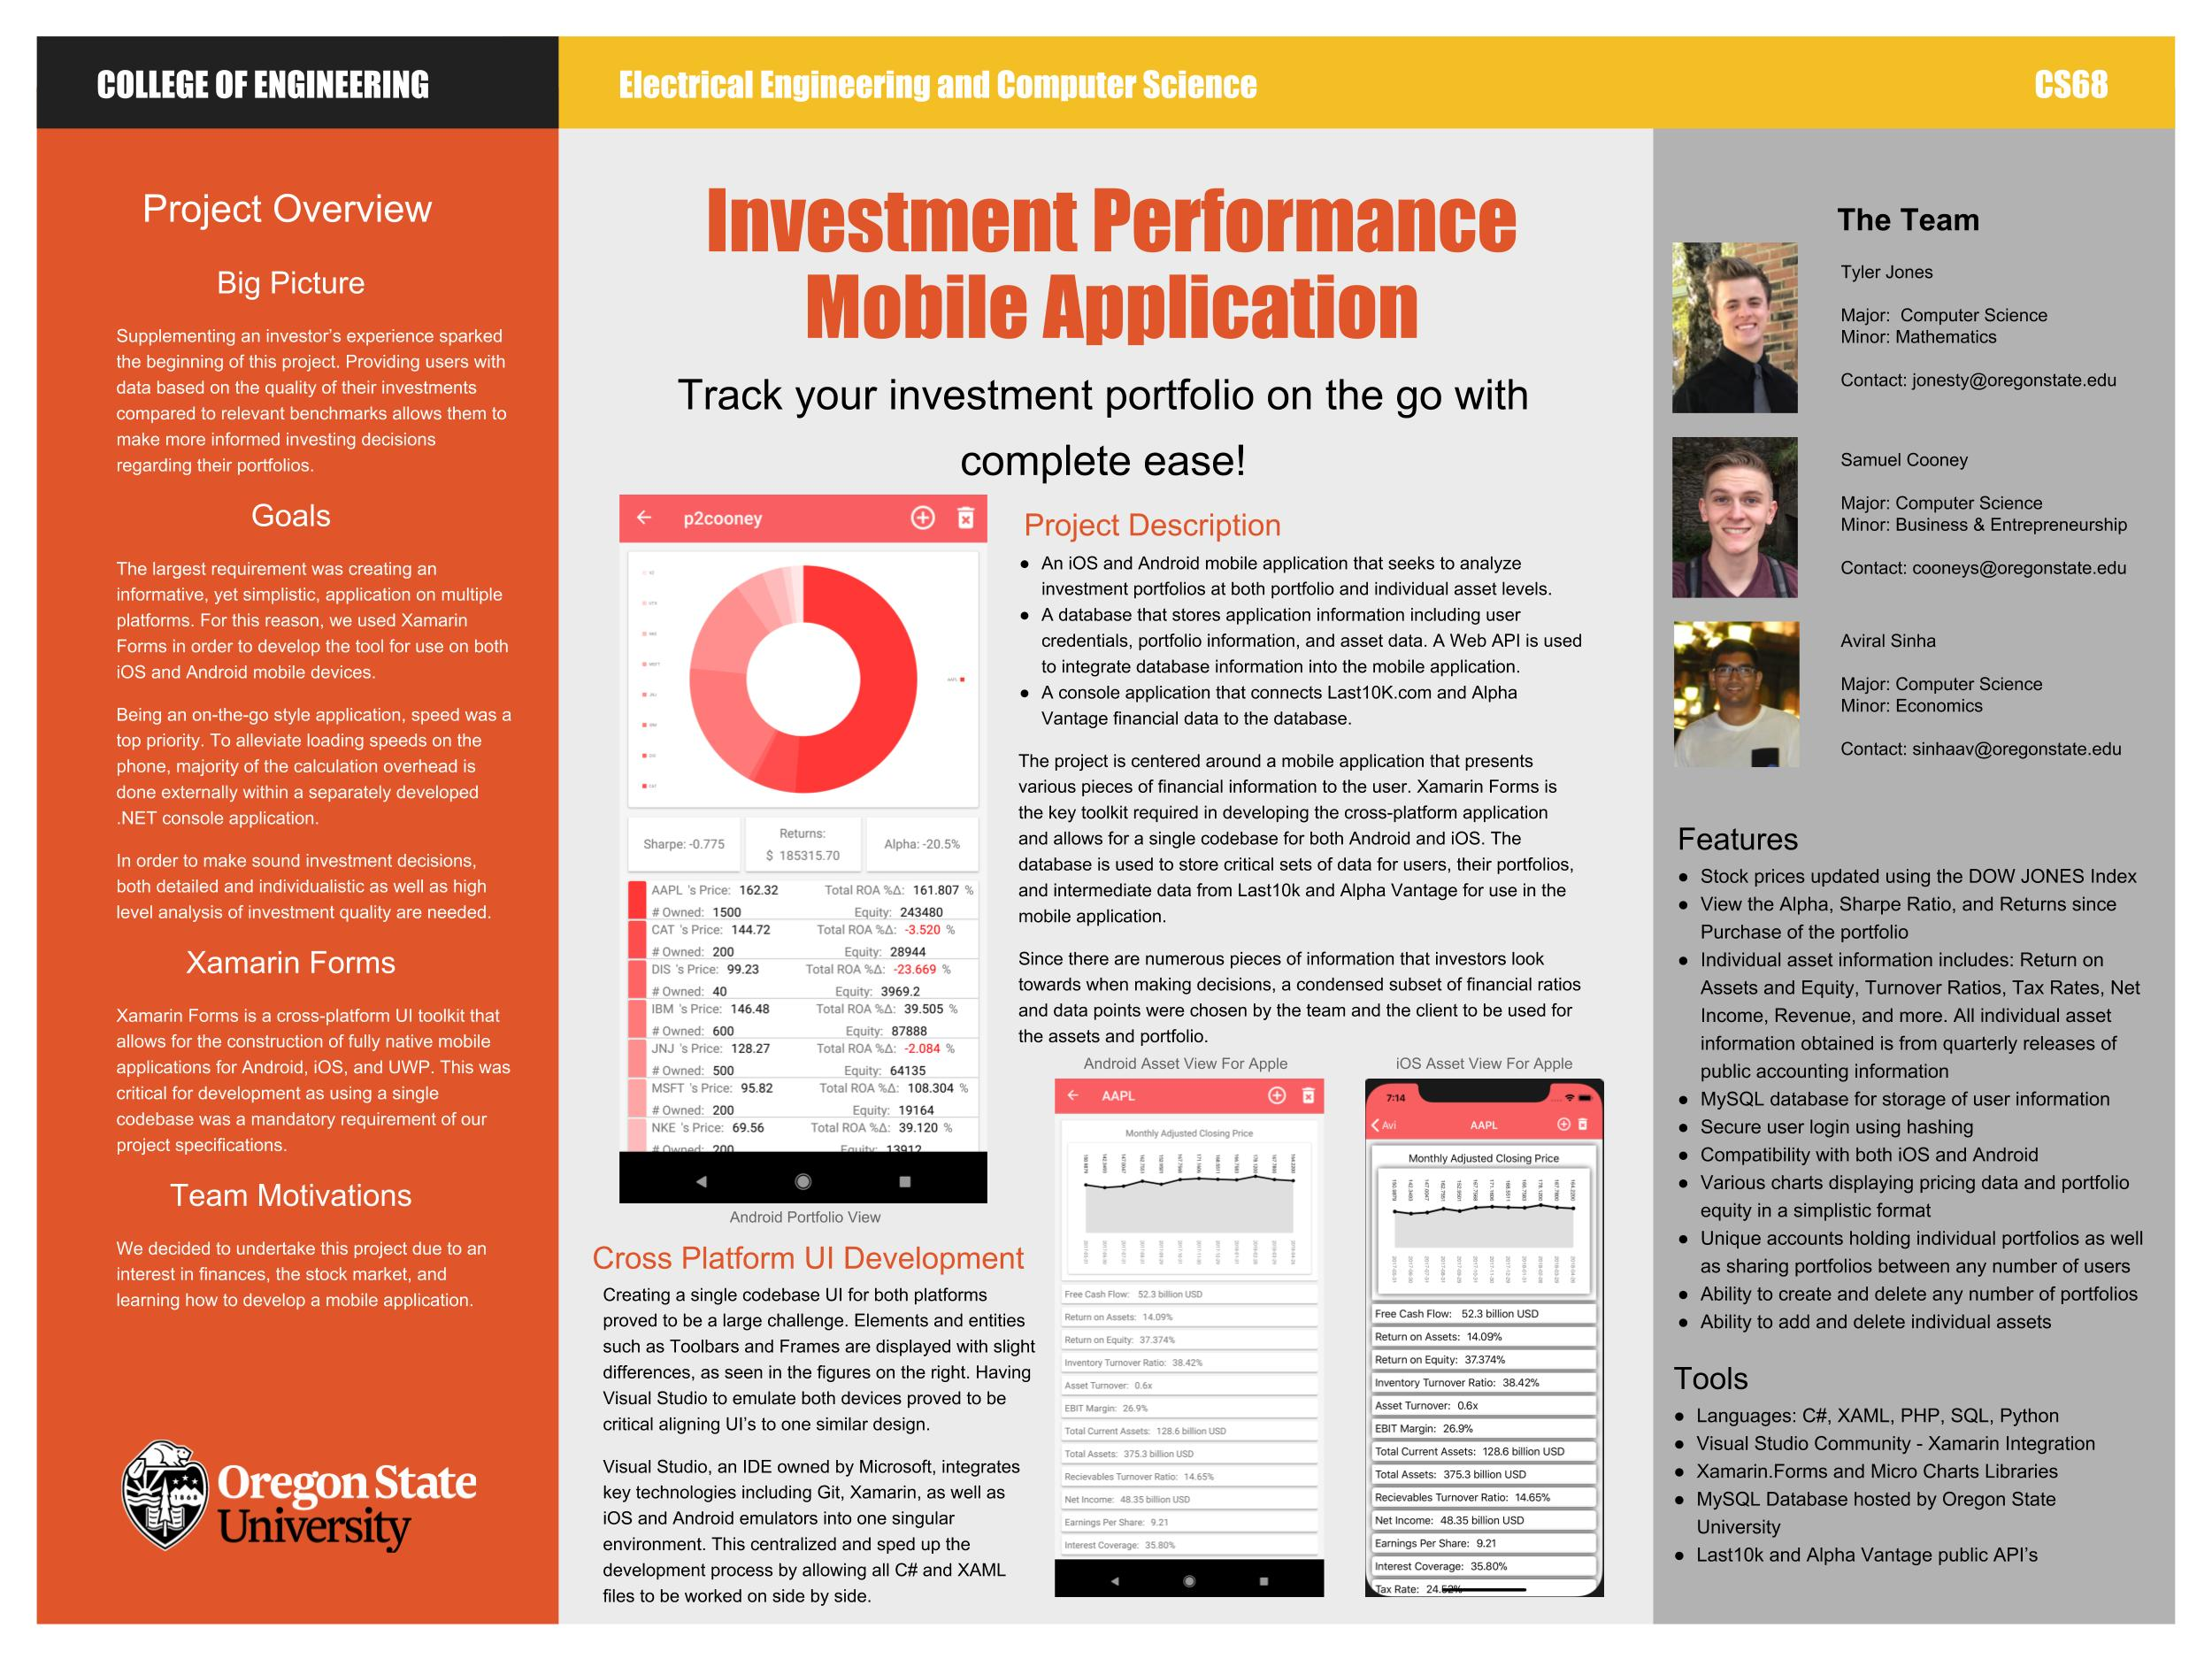
\includegraphics[scale=.25, angle=90]{poster.jpg}

\newpage
\section{Project Documentation}
\subsection{How does our project work?}
Our project is a cross platform mobile application that utilizes Xamarin. Xamarin is a Microsoft owned piece of development software that enabled us to develop our application for both Android and iOS with one unanimous code base. Rather than writing our code in Java or Swift, as would be the case of typical Android or iOS applications, Xamarin enabled us to use C\# for all of our development.

From a birds-eye view, there are 3 major components to our application. The first and most obvious is the user-facing application. The application seeks to allow users to track the progress of their investment portfolios, as well as see the performance of companies contained within their portfolio. The user has to ability to see individual data sets provided for companies that are listed in the DOW Jones index, as well as gain insight into their investment choices through the use of Jensen's Alpha, r\^2, and the portfolio's realized returns.

The remaining components of the application enable the user-facing front end to be useful. All of the user data for a given portfolio, as well as any company specific data are stored in a MySQL instance. Pricing data that is Incorporated into the calculation of alpha and r\^2 is retrieved from a third party free web API called Alpha Vantage. 


\subsection{How does one install our software, if any?}
From an installation perspective, our project can be installed on a user's actual phone if they have an Android device, or if they go through the proper procedure of uploading to the App Store or Google Play store if they have an iOS device. In the case that live deployment is not possible, it is necessary to add the NuGet packages "Avapi" and "Newtonsoft.Json" to their solution file that they download from our GitHub. The project will not run on an emulator without these packages installed. Users can easily install and uninstall NuGet packages from Visual Studio directly with the NuGet package manager.
\subsection{How does one run it?}
A user would run our application by first ensuring they have Visual Studio with Xamarin downloaded. Both pieces of software are free to download. After this, the user would simply download our .sln file and open it in a Xamarin project within Visual Studio, and begin running the emulator with a fresh build of our project.
\subsection{Are there any special requirements to run our software?}
Due to our project being a mobile application, a user would need to ensure that they have downloaded and installed a working Android or iOS emulator, depending on their native environment. If a user has an Android phone, Xamarin also supports direct deployment of the actual application onto the phone.

\newpage

\section{Recommended Technical Resources for Learning More}
Candidly, there weren't many helpful technical resources available to us, or that were needed for us to get what we needed out of our utilized technologies. Overall, as far as documentation and formal help went, Xamarin's home page and documentation, YouTube tutorial videos, and Microsoft's home documentation for asynchronous behavior proved to be more helpful than anything. There weren't too many specific, nuanced technologies that we needed a designated expert to help us with. Nearly this entire project was self taught.
\section{Conclusions and Reflections}
\subsection{Tyler Jones}
\subsubsection{What technical information did you learn?}
I learned a remarkable amount of technical information over the course of this project. Every single component of this project was a new piece of technology for me that I have yet to receive formal training in. Databases, C\#, mobile applications, asynchronous behavior, and APIs were all my main components I interacted with, and each of them was brand new to me. I had the added benefit of the fact that I also taught myself enough about each of these concepts to meet the project goals, and I think I am much better off than my peers due to the increased retention that self-teaching offers over a class room setting.
\subsubsection{What non-technical information did you learn?}
I learned that sometimes the real world is really messy and can get in the way of your goals. Repeatedly, over and over, our project took massive hits. Whether it was severe client disconnect, TA absence, or seemingly insurmountable technical barriers, it seemed that our project was doomed at times. However, I learned that facing these obstacles head on and readjusting the vision of the project when necessary is what is required in order to to complete a project that was as fragmented as ours was at times. In the real world, there are so many factors that will be out of my control as an engineer, and I will need to roll with the punches. This project has given me the opportunity to learn a great deal about myself and my work ethic when faced with such challenges.
\subsubsection{What have you learned about project work?}
I have learned that project work needs good planning. I think many things were out of my control regarding the track of the project, such as consistent client issues, but others were in my control to minimize the effect that such an issue would have on the project. I learned that by starting early, and really making sure my plan and design are thought out and sound will save me countless hours as the project progresses. I also learned that project work needs time and attention. As simple as this seems, this lesson really resonated with me as the year progressed. Unlike my other course work, which comes and goes, and is only dependent on you to complete, project work comes with a variety of other challenges that require patience and time, especially in the case where you are providing a service to an external client, and not just a professor.
\subsubsection{What have you learned about project management?}
Overall, the biggest thing I have learned is the importance of planning. Forgetting all of the misfortune that seemingly fell on our project, I feel as if the impact of such misfortune could have been minimized had I taken the planning process more seriously. Often, its difficult to put in hours of planning to something that you don't know how to do, as was the case with my components of this project, and with other outside factors demanding your attention, it is easy to shortcut the process or "just get it done". I have learned that a massive amount of time and worry can be spent on trying to compensate for the lack of planning, and the project and decisions made down the road may end up not being ideal due to the haste under which they were made. Planning is so crucial to any project, especially when typically your specs are not your own. If an outside, sometimes not technical, source is dictating the requirements of the project, it is necessary to truly make sure that you and the client understand the limitations of the software being used, and what exact goals you are seeking to meet.
\subsubsection{What have you learned about working in teams?}
Regarding project management, the biggest thing I have learned is that, ultimately, people are going to be a real limiting factor in the course of a project. Sometimes, as an individual, no matter how well or early a plan is created, team dynamics or personality types can really play an unexpected role in the vitality of the project. If one team member slacks, or feels entitled, or feels that they have done the lion's share of the work, these feelings can result in a toxicity level that can ruin the project from the inside out. I feel its necessary with project management to get a good handle on what each member is good at, and what each member is bad at, and to be candid about such answers yourself. Distributing work and managing expectations of individual team members is necessary for the health of the project to remain in tact.
\subsubsection{If you could do it all over, what would you do differently?}
If I could do this project all over, as I touched on previously, I would make sure that I knew what the project truly entailed as we went into winter term. The planning process on my end was not exhaustive enough to truly give a good sense of what was required of the project. Especially considering the nature of the components that I was responsible for being all completely new technologies, taking advantage of the allotted 10 weeks to really make sure I knew what was common practice with these technologies, how they worked, and how they could be used best to suit our needs would have saved me countless hours of stress and late nights in Winter term. Such planning mishaps as I experienced resulted in the "wrong" kind of difficult during our development process. Rather than being able to focus on the nuance of the technologies and meeting stretch goals and having a great sense of what was possible and not possible, so many hours on my end went into teaching myself how to use any of these technologies from the most basic level before I could even begin to consider thinking about how to implement them under the context of our project. This resulted in a certain kind of inefficiency and stress that I hope to avoid at all costs going forward with future projects.

\subsection{Aviral Sinha}

\subsubsection{What technical information did you learn?} 
I learned a lot about software and mobile development, agile development, version control, REST APIs, C\# and SQL.

\subsubsection{What non-technical information did you learn?} 
I learned a lot about combining finance with software development. Portfolio and Asset level calculations being taken from their native excel environment and adapting them into our environment for the application.

    
\subsubsection{What have you learned about project work?} 
I learned a lot about working with various other parties both in the immediate development group as well as with a boss(client) and other significant individuals(TA). We were able to delegate work properly and it was up to us to set deadlines and make progress and complete the project by the time it was expo. 
    
\subsubsection{What have you learned about project management?} 
My skills in project management only improved with capstone. I learned how to manage tasks that I had weekly as well as delegate tasks. I learned how to properly use tools like github and slack  to make sure all of our work was able to stay on track and we could see each others progress.
    
\subsubsection{What have you learned about working in teams?}
Working as a team I learned a lot about how dynamics can be affected over the course of a year and how we have to constantly be planning ahead. Our issues with the client through the year caused a lot of distress as they kept on disappearing so we had to constantly communicate among each other so the project could progress and be completed 
    
\subsubsection{If you could do it all over, what would you do differently?}
If we could do it differently then I would definitely have started development either fall term or during winter break because while 10 solid weeks of development is enough time having extra time in the end to debug any issues would have been very helpful. I also should have done more research in what APIs we were using because none of the ones we chose in fall term seemed viable for our final product. Our client recommended Quandl but the data needed from the service was only available to premium members and our visualization tool was replaced with Xamarin’s own charts tool which we learned about as we understood Xamarin even more. 

\subsection{Samuel Cooney}
Being new to mobile development, database work, and visual studio, I learned many new languages during this project. XAML is a markup language that was used to develop majority of the User Interface elements
displayed in  the application. C\# was used to create the front-end logic and also created some of the UI elements. SQL and PHP was learned to allow users the ability to delete assets and portfolios from their
account. Besides languages, I learned about integrating databases with consol and web applications as well as with a running mobile application.
I also learned how valuable comments in code were, as sometimes I would be refactoring work from a few months prior and if I forgot to include comments, I had to spend extra time refreshing myself to my previous work. 
Some of the more non-technical skills I learned during this project were mostly management related. I learned to set weekly goals and progress checkups for myself and my teammates which I used to 
believe was implicit in working with a team. I also discovered that not everyone has the same understanding on professional relationships and how they should be handled and sometimes
I will have to take the lead on establishing such connections. Finally I understood that issues between the team need to be brought to light immediately 
and consequences need to be set ahead of time, so the whole team is on  the same page with what is going on. This was an interesting take on project work as
I have never been in a role of the project manager, only a developer on a project team, and so to balance both roles while maintaining balance with Tyler's managerial skills
proved to be an interesting and fulfilling learning experience. If I were to redo this project, besides being more upfront about team commitment and responsibility, I would
focus more of my work on the front end of the project. Spacing development work to just Winter and Spring terms proved to be a large portion of stress and I would begin development
or at least learning of the tools during Fall term.


\end{document}
